%!TEX root = first try.tex

% \chapter{Case study}

% A case study to assess the feasibility of the methods/criteria developed in previous paragraphs by using both FEM software and methods/criteria. 


\chapter{Conclusion}

%Compare the result from different calculation method. Give conclusion based on the comparison result.

\begin{appendices}

\chapter{Investigation of report series created by D181 Committee Group}

D181 Committee Group is created by UIC, in order to investigate Lateral Forces on Railway Bridges. Some of the proposed criteria in reports created by this committee group are adopted by Eurocode Committee to created Eurocode 1991-2.

\section{Structure of report series}

Reports involved in the series are listed below in the order of publishing time:

\begin{enumerate}
    \item RP 1: Summaries of national standards and literature survey
    \item RP 2: Submitted programs and example of application
    \item RP 3: Dynamic measurements on the steel bridge over the Brenta river on the MilanVenice line at 234 + 0.963 km
    \item RP 4: Dynamic measurements on steel bridges over the Váh river by Sala on the MarcheggSzob line at 117 748 km
    \item DT 312: Etude de l'influence de la fréquence du filtre sur les valeurs mesurées des forces verticales et latérales sur les rails
    \item RP 5: Dynamic measurements on the metal arched bridge on PKP
    \item DT 313: Analyse des déformations latérales d'un pont souple (cas du PONT de LIXHE) Ligne SNCB de TONGRESMONTZEN par J.J. REBER SBB Bau GD
    \item DT 329: Parametric study Part 1: Parametric study Initial phase (September 1994) Part 2: Parametric study Phase 2 (February 1995) Authors: L.T. James and G.A. Scott
    \item RP 6: Final Report
\end{enumerate}

In this thesis DT 329 and RP 6 are obtained and studied, but other reports in English version are not available to the researcher.

\section{Items of interests in report series}

1. The proposed 1.2 Hz Criterion and its background. It is discussed in RP6.

2. Resonance mechanisms studied. They are discussed in DT329.

3. Lateral forces on the bridges

\section{Resonance mechanisms studied in DT329}
\subsection{Methodology of Parametric Research DT329}

The research was conducted in two phases.

For the initial phase, the dynamic lateral response to the passage of different train types of various theoretical bridge models are to be examined using VAMPIRE. The method of modelling bridge behaviour adopted is the Theory of Normal Modes. Each train is modelled as a series of masses interconnected by suspension components of known characteristic. Time-step integrations are then performed to simulate the passage of a train over the bridge model along a track sample, which extends beyond the bridge.

Comparisons of measured bridge responses with VAMPIRE simulations of the bridges and trains involved were the subject of earlier studies for ERRI Committee D 181, the results being documented in reports RP 3, RP 4, and RP 5 of the Committee. Each vibration model was derived from finite element analysis of the bridge structure.

The committee have selected eleven sets of bridge parameters to be subjected to a selection of lateral load conditions. Lateral loading is provided by three train types, each running at two speeds within their respective operational ranges, on track appropriate to the train type. The combinations selected for this phase are tabulated in Appendix 1. Since the bridge design parameters are necessarily general, finite element techniques for producing bridge vibration models are inappropriate; general transverse beam vibration theory is used instead.

For the secondary phase, as part of ERRI(UIC) investigation of Lateral Forces on Railway Bridges, the ERRI D181 Committee have commissioned British Rail Research (BRR) to carry out a parametric study(DT329) using their VAMPIRE dynamics software. 

The study has investigated the influence of key bridge parameters and of different train types on the lateral deflections and lateral forces exerted on the bridge. The study has been carried out in two phases.

The first phase examined 52 combinations of bridge parameters and train configurations. This study showed that some of the input parameters had little influence on the dynamic behaviour of the bridge and that others had a significant influence. There were also some parameters which appeared to show resonant effects at particular values. The results were presented in the initial report (Reference [1], part 1 of this ERRl D 181/DT 329).

From the results of the first phase of the study, the ERRI DI81 Committee were able to select the cases for the second part in order to concentrate on those parameters which had the largest influence on the behaviour of the bridge. The cases to be considered were divided into three categories. These investigated the influence of multiple span bridges (viaducts), the influence of track quality and the influence of stiffness/span/frequency on the resonant behaviour of the bridge.

It is noted that all studies were done using VAMPIRE software, which is a computer program aiming to simulate running train vehicle behaviour. The reliability of simulation has been discussed and confirmed in RP2: Submitted programs and examples of application. However, this thesis doesn't have any insight into this report since it's not available to the researcher. 

Focus is placed on secondary phase of study of DT329, since it consists research on resonance behaviour of the bridge.

\subsection{Model of bridge}
The bridge cases were modelled by assuming the bridges to behave as simply supported uniform beams. Transverse beam theory was then used to determine the frequencies and mode shapes of vibration for a given combination of span, mass per unit length and flexural rigidity. The modal information for the bridge was then used in a 'Normal Modes' analysis of the bridge.

For each case, all lateral modes of vibration up to and including 20 Hz were used. In order to prevent this artificially over-simplifying the model, if fewer than five modes were 20 Hz or less, all of the first five were used.

\subsection{Bridge parameters}

The spans to be considered are: 20 m, 33 m, 54 m, 90 m and 120 m. The flexibilities, defined as deflection of mid span over span length due to a static point load of 100 kN at mid span, are: 114000, 1/10000, and 1120000. The mass per unit lengths required are: 2 tonnes/m, 6 tonnes/m, and 10 tonnes/m.

\subsection{Vehicle parameters}
Three train types are considered: a typical freight train, a typical standard passenger train, and a typical high speed passenger train. Appendix.\ref{app:dt329data} details the parameters used to construct each model. In general, each model consists of a locomotive and a number of identical vehicles appropriate to the train type. The total number of axles in each train is 24. Although effects on the train are only examined on the first vehicle of each type, extra vehicles are added to the train to see what cumulative effects occur to the bridge.

The freight train consists of a British Railways Class 56 locomotive and nine UIC wagons. This has a total length of 131.56 m, which assumes a nominal vehicle coupling distance of 4 m. Runs at 60 km/h and 100 km/h are required.

The standard passenger train consists of an E444 locomotive and five UIC coaches. This has a total length of 143.8 m. It is based on one of two train models used as part of the study of the FS Bridge discussed in report RP 3 of the Committee, differing only by the addition of three extra coaches. This is required to run at 160 km/h and 200 km/h.

The high speed passenger train consists of an ETR500 locomotive and five ETR500 coaches, having a total length of 145.8 m. It is based on the other FS bridge study train model mentioned above, differing from the original by an additional three ETR500 coaches. It is required to run at 300 km/h and 350 km/h.

\subsection{Track}

For initial study phase, the track samples used were consistent with each train type. PSD plots of each are shown in Figures \ref{fig:track1} to \ref{fig:track3}. Sample TRACKFRT.DAT was used for all analysis runs for the freight train. This is measured data from a typical BR freight line. Sample TRACKPN.DAT was used for the standard passenger train analysis runs. This is measured data from a part of the BR East Coast main line. Sample TRACKPH.DAT was used for high speed passenger train analysis runs. This is measured data from a typical DB high speed line.

Samples of 500 m were chosen so that there would be 100 m before the bridge and at least 100 m after the bridge for all combinations of span and train length. The initial 100 m is required to check vehicle behaviour on the track irregularity alone, and the portion after the train has left the bridge is required to check that the bridge vibrations decay.

For secondary study phase, the track data used to excite the mathematical models was taken from the British Rail Research library of measured track data. For the viaduct and resonance investigations, the track files used were the same as those used in the first part of the study. For the investigation of the influence of track quality, additional track data was used so as to give the widest possible range of realistic track qualities.

\subsection{Contact data}
For each run the same contact data was used, consisting of rails inclined at 1:20, and wheel profiles of conicity of 0.05 (based on standard British Rail 113A rails and PI wheel profiles). The coefficient of friction applied was 0.3.

\subsection{Summary of modelling procedure}
The modelling of simulation for most of the research purposes of both phases generally used a routine where bridge module and same train-type-coupled track irregularities, vehicle parameters were adopted. That means the parameters of track and vehicle are exactly the same among all simulations are the same if not specially noted. This frequently used simulation set-up will be called routine in the following paragraphs. See previous sections for detailed information about routine.


\vspace*{\baselineskip}
The routine is used in following researches:
\begin{enumerate}
    \item Phase I: All research on bridge parameters
    \item Phase II: Viaduct study
    \item Phase II: Resonant study
\end{enumerate}

\vspace*{\baselineskip}

Track quality study in secondary phase which used different simulation set-ups. The following trains:

Freight 60 km/h 

Freight 100 km/h 

Freight 120 km/h 

Passenger 200 km/h 

High Speed 350 km/h

were run, each with 3 different conicity values (0.05, 0.2 and 0.4) over 14 sections of measured track data each of length 1 km.


\subsection{Data produced}

For every analysis run the following results were obtained at intervals of 0.01 seconds.

BRIDGE DATA:

Lateral displacement at mid span Lateral acceleration at mid span

\vspace*{\baselineskip}

VEHICLE LATERAL ACCELERATION DATA:

Loco body at leading pivot

Leading coach/wagon body at leading pivot/axle Loco leading bogie

Leading coach/wagon leading bogie/axle

\vspace*{\baselineskip}

TOTAL LATERAL FORCE DATA:

Loco leading bogie

Leading coach/wagon leading bogie/axle

\vspace*{\baselineskip}

LATERAL FORCES ON INDIVIDUAL WHEELS

Leading coach/wagon, first axle, left and right wheels 

Leading coach/wagon, second axle, left and right wheels 

Loco, first axle, left and right wheels

Loco, second axle, left and right wheels

\vspace*{\baselineskip}

In addition, for freight train runs, since the locomotive has two bogies of three axles, the forces on the individual wheels of the third axle were also produced.

Peak values for each of the outputs produced for the required ranges were obtained. For bridge outputs, peak values were taken for the period where any part of the train was on the bridge. For loco and leading coach/wagon outputs, peak values were taken whilst the vehicle in question was in contact with the bridge.

Peak values for each output were then read into a spread sheet where they could be compared more easily to check for emerging trends. The spread sheet has been partially automated to produce graphs of a single output for each train type for a single varying bridge parameter, for given values of the other bridge parameters. Figures 4 to 30(\cite{d181dt329}) show typical plots which have been produced in this manner.

\subsection{Resonance caused by axle repeat pattern}

Axle repeat patterns are wavelength phenomena - regardless of vehicle speed, the repeat length is constant. However, since frequency is speed divided by wavelength, the frequency of the axle repeat patterns vary with train speed. A table of axle repeat pattern lengths, and typical frequencies arising from train speed are given in Figure.\ref{tab:329axlerepeat}

By running train in different speeds shows resonance is possible between train and bridge if the axle passing frequency coincides with the first lateral bridge mode, the effect occurring in bridge lateral displacement over a limited frequency range around the resonance frequency.

However, the speed on theory which should yield resonance effect may be different from the speed that actually triggered 

\subsection{Resonance caused by kinematic movement of trains} 
Kinematic wavelength also gives rise to frequencies which vary with speed for the same reason. For first lateral bending mode coincidence with kinematic frequency, the kinematic wavelength of each train type had to be established, by running each train at a range of typical operating speeds over a discrete lateral irregularity, and examining the frequency content of the lateral wheel motion. The resulting wavelength ranges are tabulated in Table.\ref{tab:329kinematicwavelength}. 

The most likely possible resonance in the initial studies to be of this type was between the passenger train at 200 km/h (55.556 m/s) on passenger track and BR PI wheel profiles, and a span of 54 m, stiffness 1/10000, mass/length of 6 tonnes/m. This combination was examined by varying the speed between 55.556 - 64.6 m/s over the span, and by varying the stiffness of the span between 117000 and 1112000 running the train at 55.556 m/s. Another combination was examined - the ETR500 train running between 65 - 80 m/s on high speed track and BR PI wheel profiles, for a span of 38 m, stiffness 1110000, and mass/length 10 tonne/m; the span in this case was chosen to coincide with the kinematic wavelength of the coaches.

Coincidence of vehicle kinematic frequency with bridge first lateral bending mode may cause resonance to occur over a broad range of frequencies to a less pronounced effect than coincidence of axle passing frequencies. Evidence of coincidence of kinematic wavelength with length of span has been found in the lateral acceleration of bridges, but was not demonstrated in the lateral bridge displacement in the cases examined. For short kinematic wavelengths, this effect could not be seen, possibly because of lack of time for the bridge to respond.

\subsection{Apparent shift in resonance frequency}
It is frequently observed in the output of both resonance effects that apparent resonance happens at some frequencies higher than frequencies calculated on theory. This is explained in following quote on \cite[Page 13, Secondary Phase]{d181dt329}

\begin{quote}
Although the peak mid span displacement was expected to occur at 28.5 mis, it can be seen that for the runs with just the coaches that the peak occurs at about 32 m/s. This is confirmed to be a resonance-type effect rather than a discrete event in the time histories of the runs, a selection of which are shown in Figure C6(Original report), of which an extract of 100-285m follows as Figure C7(Original report). This speed is mid way between axle passing frequency coinciding with first bending mode of the bridge, and kinematic frequency coinciding with the first bending mode. So, the apparent shift in resonant frequency may be due to a combination of these effects (see discussion of kinematic frequency resonance results). However, an alternative explanation may be that as track forces generally increase with speed, the deflection of the span would be expected to increase. If this effect continued through a resonant band, the peak displacement would appear greater at a speed slightly above that calculated for resonance, as sketched in Figure \ref{fig:apparentshift}.
\end{quote}

\begin{figure}[h]
    \centering
    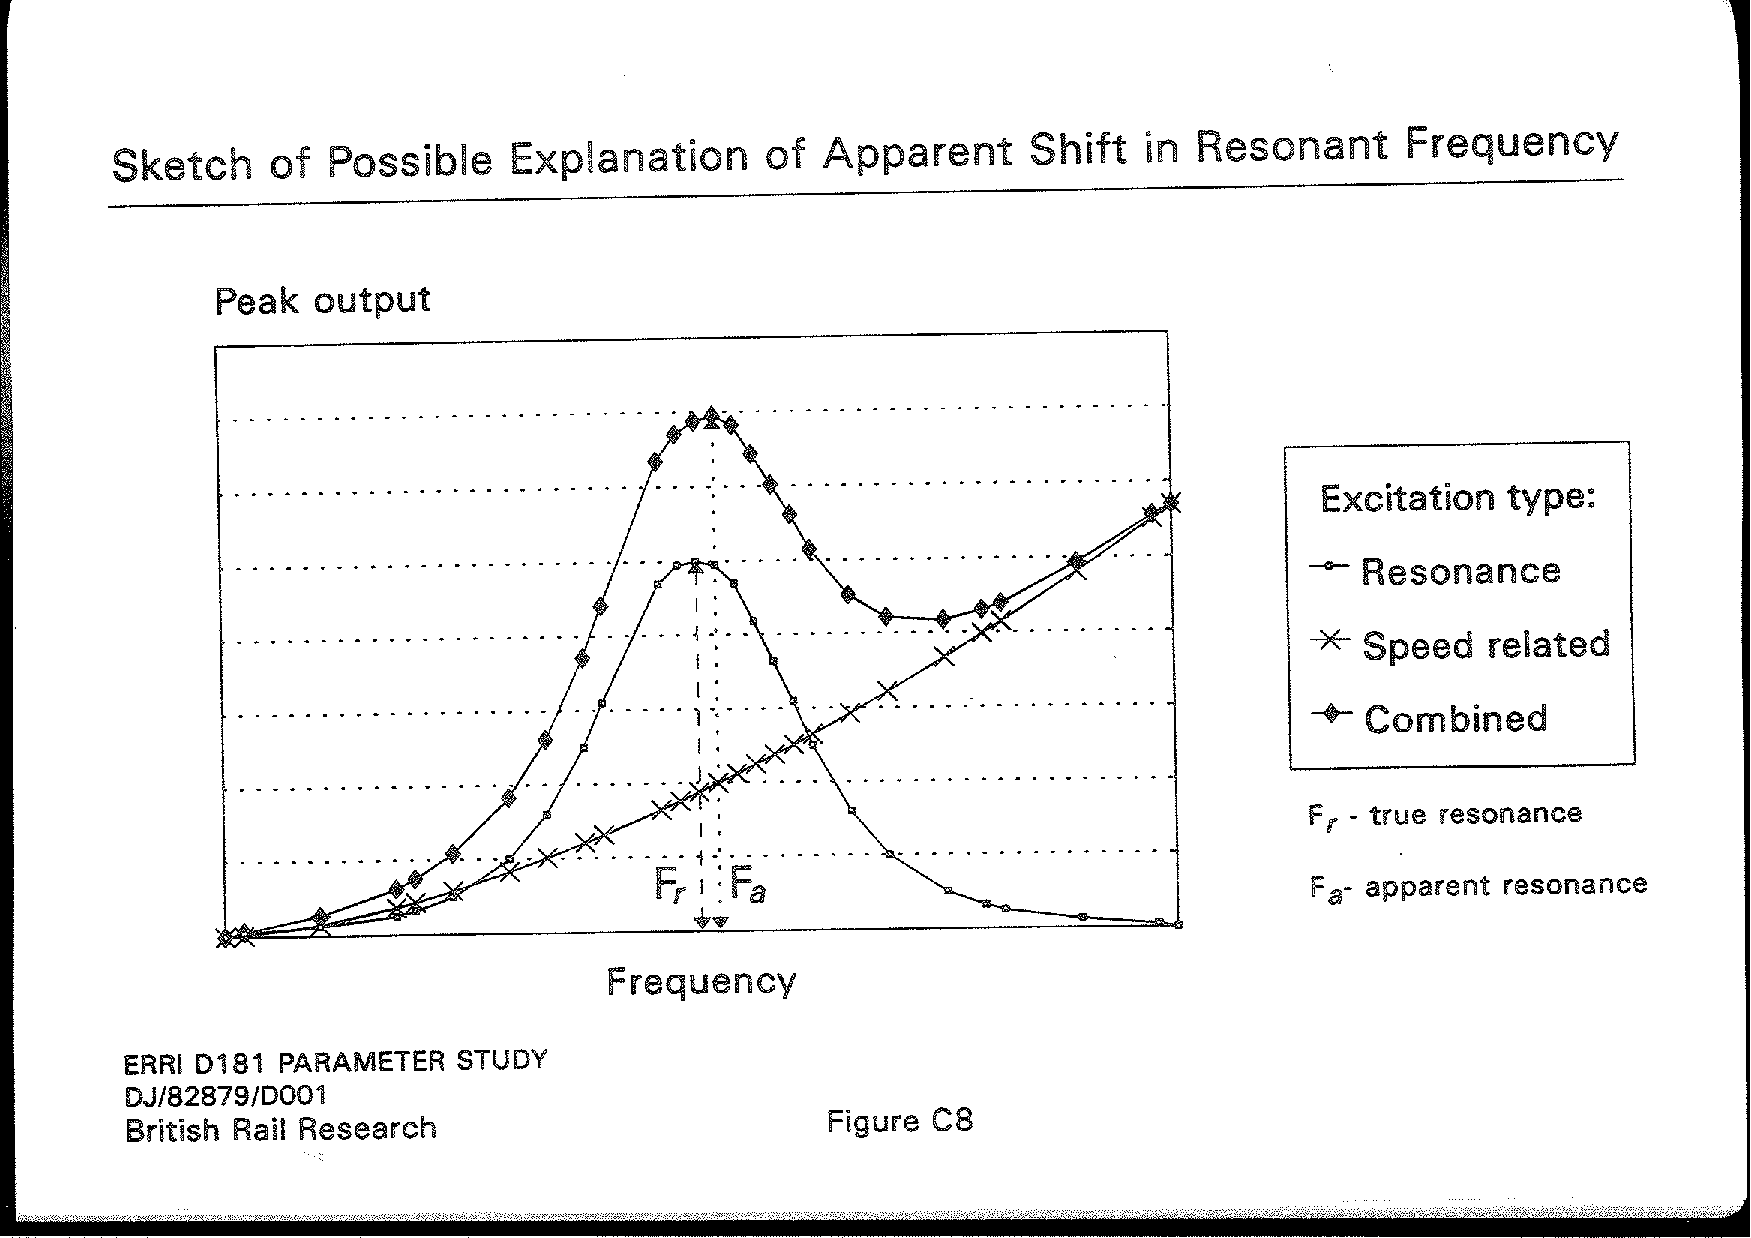
\includegraphics[width=\textwidth]{apparentshift}
    \caption{Sketch of Possible Explanation for Apparent Shift in Resonant Frequency. Extract from \cite[Appendix 2]{d181dt329}}
    \label{fig:apparentshift}
\end{figure}

What's more, track irregularities profile in normal analysis runs may also contribute to resonance shift. This is due to the wavelength on theory is obtained by an analysis run adopting a discrete irregularity, which is different from those analysis runs yielding apparent resonance shifts. And theory resonance frequency is calculated on the wavelength output of this specific run. 

Both explanations indicate that apparent resonance frequency can hardly be predicted. Apparent frequency may even shift into domain lower than theory frequency. 


\section{Debate on proposed 1.2Hz Criterion in RP6}
Evidence of \cite{d181} is the origin of \cite[A.2.4.4.2.4(3)]{EC12} is found in \cite[p4.2: Lateral Frequencies]{d181}:

In order to avoid the phenomena of lateral resonance in vehicles, the first natural frequency of lateral vibration of the span $f_{lt}$ such that:

\begin{equation}
f_{lt} \geq 1.2Hz
\end{equation}

The statement exactly coincides with criterion A.2.4.4.2.4(3) in Eurocode 1991. It is sufficient to acknowledge D181 RP6 as the origin of criterion A.2.4.4.2.4(3) because this report is created by UIC.

The value of frequency limit, 1.2Hz is explained in \cite[p3.2: Criterion 2]{d181}:

\begin{quote}
To avoid the occurrence of resonance in the lateral motion of the vehicles due to the lateral motion of the bridge, a limit value lower than the first natural frequency $f_1t$ of the lateral vibration of the span studied should be fixed. The natural frequency for lateral movements is between 0.5 and 0.7 Hz for coaches and between 0.7 and 1 Hz for locomotives. We therefore propose a safety margin $F_{lt} \geq 1.2Hz$
\end{quote}

The original author of report RP6 Graham Scott was contacted to reveal the background of 'natural frequency for lateral movements'. Mr.Scott is still in charge of the development of software VAMPIRE and he's still active in the field. Unfortunately he was unable to remember what did 'natural frequency for lateral movements' stand for in previous quotes since it was written nearly 20 years ago. He passed me to his colleague Alan Minnis for further questions. Mr.Minnis stated following:

\begin{quote}
Looking at the values I think they would refer to typical rigid body modes of a vehicle.  These are independent of speed and a typical passenger coach with air suspension will have a lower sway frequency of around 0.6Hz which is within 0.5-0.7Hz.  Locomotives tend to have a slightly stiffer suspension hence the slightly higher frequency range.
\end{quote}

Mr.Minnis statements, combined with results yielded in supporting parametric report DT329 proves 1.2Hz criterion isn't sufficient in avoiding the occurrence of resonance between train and bridge structure, nor it's sufficient in providing safety to the bridge. The reason is listed below:

\begin{enumerate} 
    \item There is lots of evidence can be found in report DT329, showing resonance can happen on a bridge with a first lateral natural frequency even higher than 1.2Hz, which is self-conflicting with 1.2Hz criterion. For example, \cite[Page 14,Phase II]{d181dt329} shows resonance occurs on 1.71Hz:
        \begin{quote}
            The first lateral bending mode of this bridge is at 1. 71 Hz. The kinematic wavelength of the passenger coaches is around 34-38 m, giving a kinematic frequency range of 1.46 - 1.63Hz.Speeds of 58.14 m/s(1.53-1.71 Hz)and 64.6m/s(1.7-1.9Hz)were also done. The mid span lateral displacement for each of the time histories are shown in Figure C12(Orignial report). The slowest speed appears to show the greatest resonance.
        \end{quote}
    \item The resonance between rigid body mode of train and first lateral vibration mode of the bridge has never been discussed in all D181 report series. No research proofed this kind of resonance can happen in real life scenario.
\end{enumerate}

\section{Lateral forces on railway bridges}
It is concluded in initial phase of the study that presence of the bridge doesn't influence the track forces and track quality is a major factor in determining the lateral forces generated by a particular train on \cite[Page 7, Secondary Phase]{d181dt329}

\begin{quote}
    From the initial study [1], it was concluded that the track quality on a bridge is a major factor in determining the lateral forces generated by a particular train. The D181 Committee therefore asked BRR to determine the peak track forces generated over a wide range of track qualities.

    The length of a bridge is small compared to the overall length of a railway track and so track quality on a single bridge may not be representative of that on other bridges on the same route. However the initial study concluded that, in general, the lateral track forces are not influenced by the presence of the bridge.
\end{quote}

The resonance effects mentioned in the previous sections were only observed in deflection and acceleration domain due to the reason that the presence of the bridge doesn't influence the track forces. 

The output of track forces from track quality study was used to create a loading model for proposal in RP6. The lateral forces are given as characteristic values $F_m + 3s$, $s$ being the standard deviation. Lateral forces from vehicle/bridge interaction as a result of hunting are presented in \cite[Page 33]{d181}. To illustrate, a sample of load model is presented in Figure \ref{fig:lateralloadcasesample}. See \cite[Page 33]{d181} for detailed usage of each load model. 

\begin{figure}[h]
    \centering
    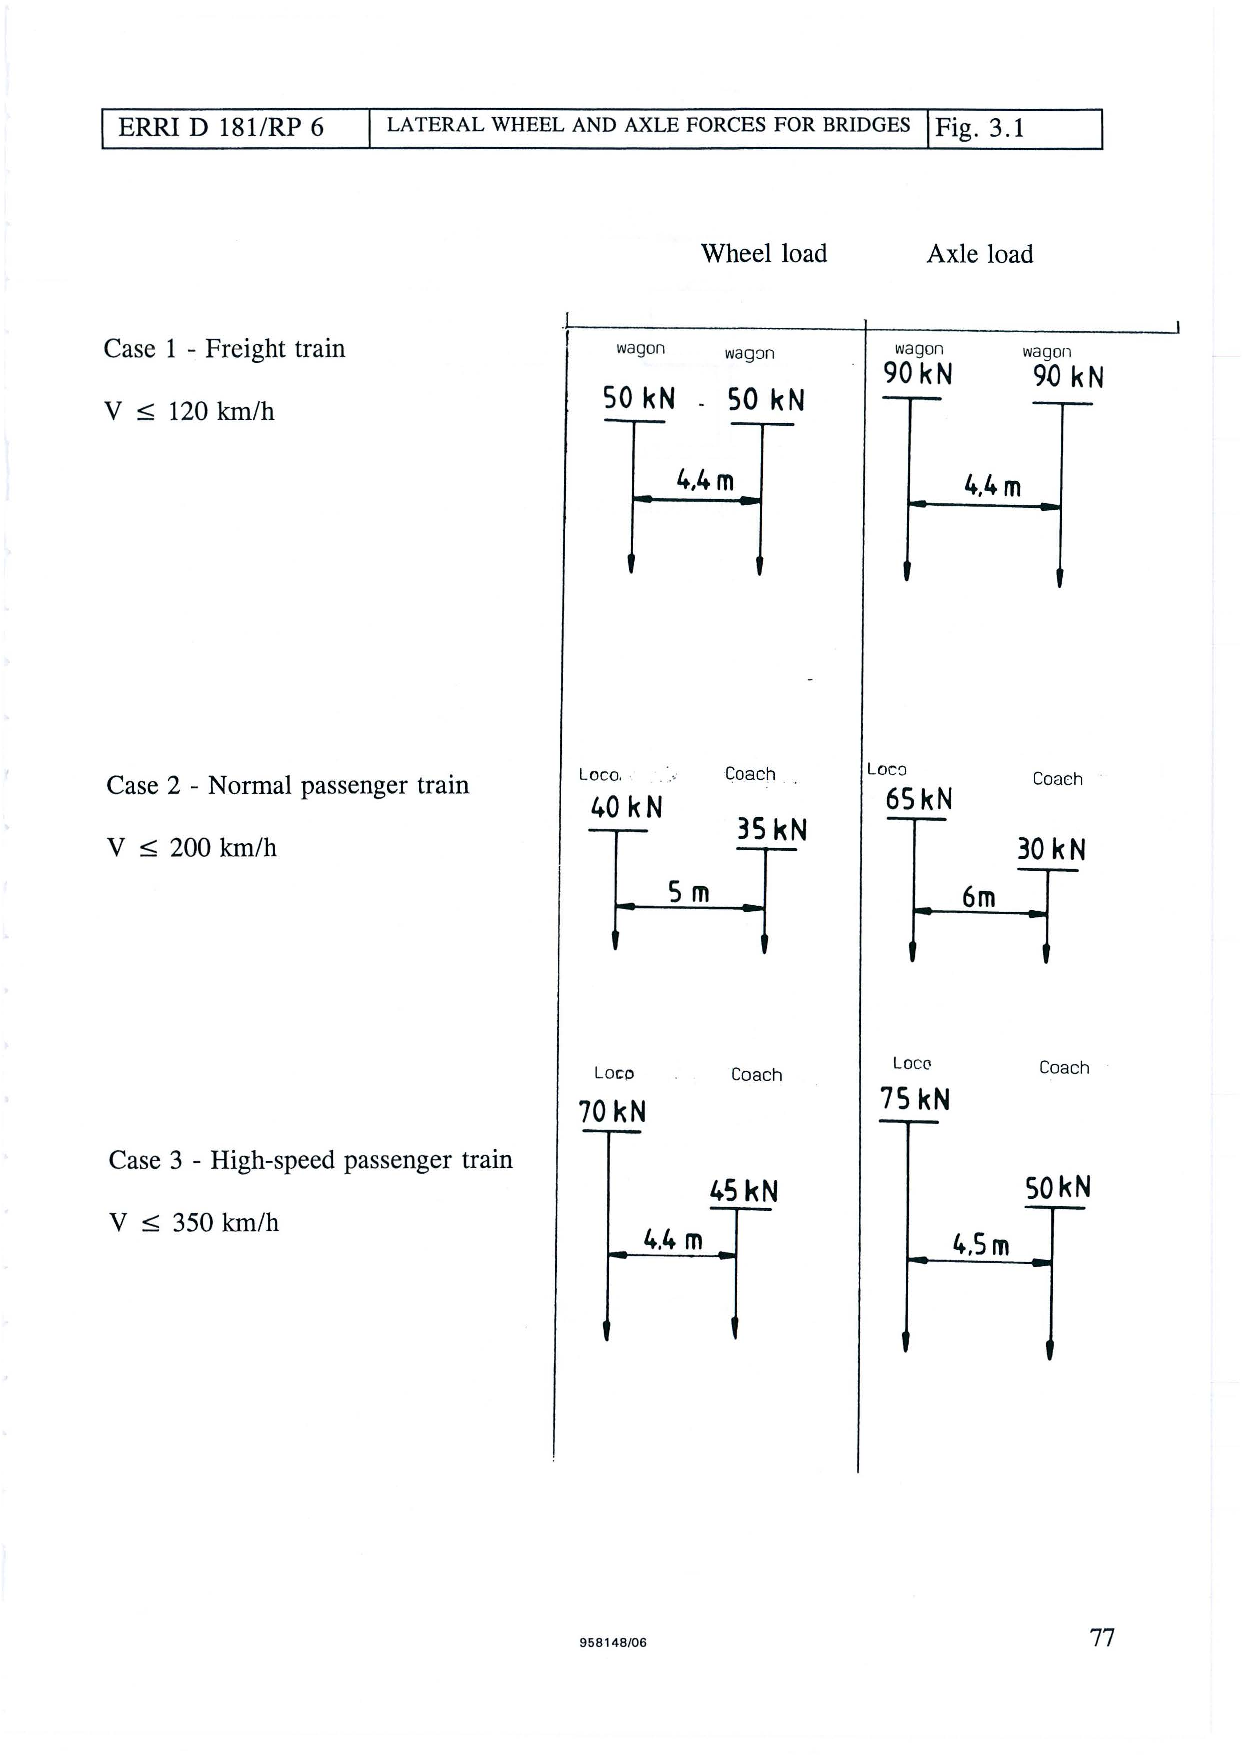
\includegraphics[width=\textwidth]{lateralloadcasesample}
    \caption{LATERAL WHEEL AND AXLE FORCES FOR BRIDGES. Extract from \cite[Fig 3.1]{d181}}
    \label{fig:lateralloadcasesample}
\end{figure}


\section{Summary of D181 report series}
The report series managed to create load models for lateral dynamics railway effects. It is worthy to note that the lateral force on the track wasn't influenced by the presence of the bridge. The major influencing parameter for lateral force is track quality and conicity of the wheel profile. 

The resonance phenomenon was successfully reproduced and observed, though its only visible in deflection and acceleration domain. A basic characteristic of resonance, regardless of resonance type, is apparent resonance frequency will shift from resonance frequency calculated on theory. The shift is unpredictable in the sense of both direction and magnitude. The effect related to speed start to creep in when speed is higher, making the effect of resonance less pronounced in higher speed(Figure \ref{fig:apparentshift}). 

Please note that every bridge will always have resonance with running train because axle repeat pattern and kinematic movement are both wavelength phenomenon, which means there is always a speed of train yielding a vibration frequency coincides with the first lateral natural frequency of bridge. However, the effect of resonance happening on long-span bridge is usually unpronounced since the speed of the train is low as 2.5m/s to 14m/s when resonance occurs.  

Some of the conclusion and proposed criteria in RP6 were adopted in Eurocode 1991-2.It is proofed that 1.2Hz criterion was adopted without amending. However, most probably load cases created by RP6 was amended before being adopted into \cite[A6.5.2]{EC12}, since there exists slight difference. 

The 1.2Hz criterion was under debate and proofed unreliable in fulfilling its original intention, avoiding occurrence of resonance. There is no research in D181 report series supporting this criterion, nor there exists literature behind the natural frequency of vehicles. This criterion ignored the possibility of future bridge designs with long span would certainly have a natural frequency lower than 1.2 Hz. It is advised that Eurocode review this criterion and revise it.


\chapter{Plots and diagrams used in D181 DT 329}\label{app:dt329data}

\begin{figure}[h]
    \centering
    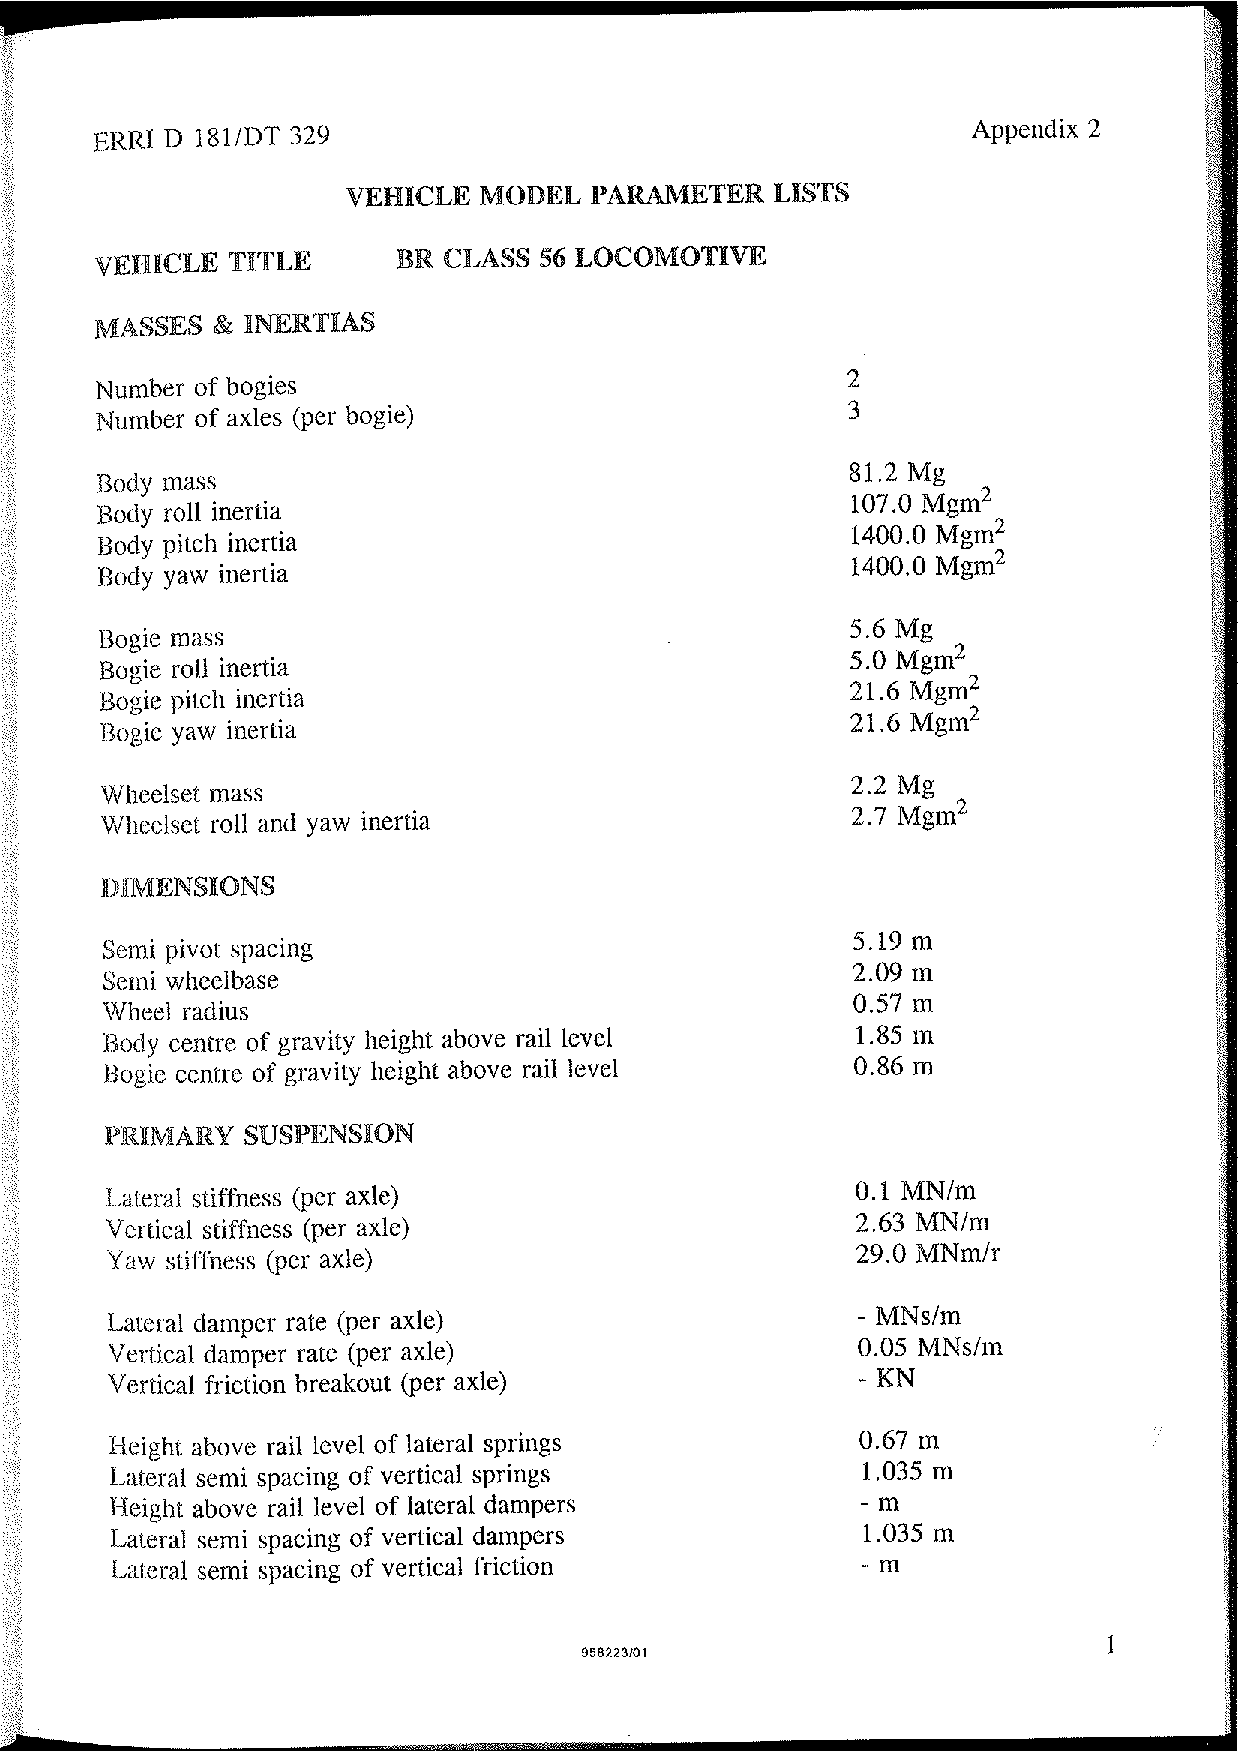
\includegraphics[width=\textwidth]{vp11}
    \caption{BR CLASS 56 LOCOMOTIVE. Extract from \cite[Appendix 2]{d181dt329}}
\end{figure}

\begin{figure}[h]
    \centering
    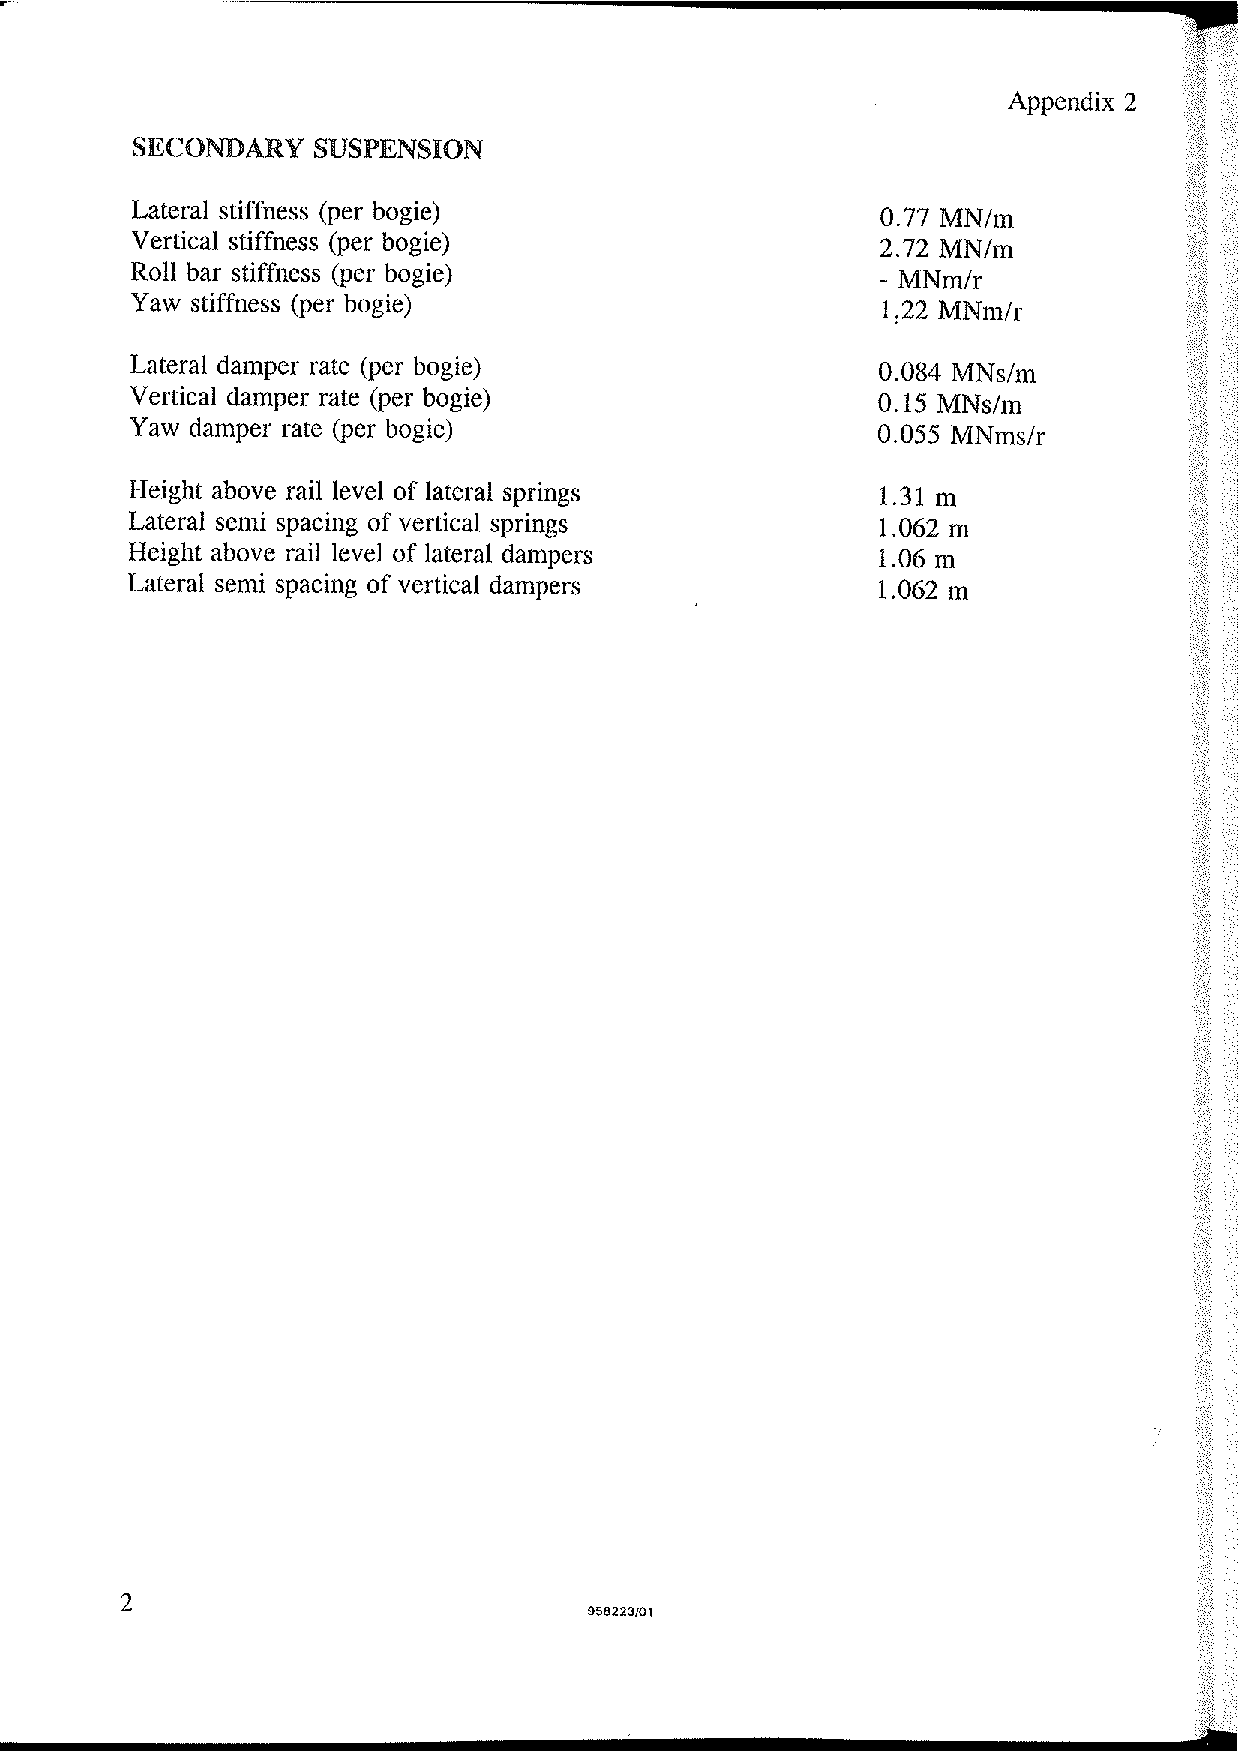
\includegraphics[width=\textwidth]{vp12}
    \caption{BR CLASS 56 LOCOMOTIVE. Extract from \cite[Appendix 2]{d181dt329}}
\end{figure}

\begin{figure}[h]
    \centering
    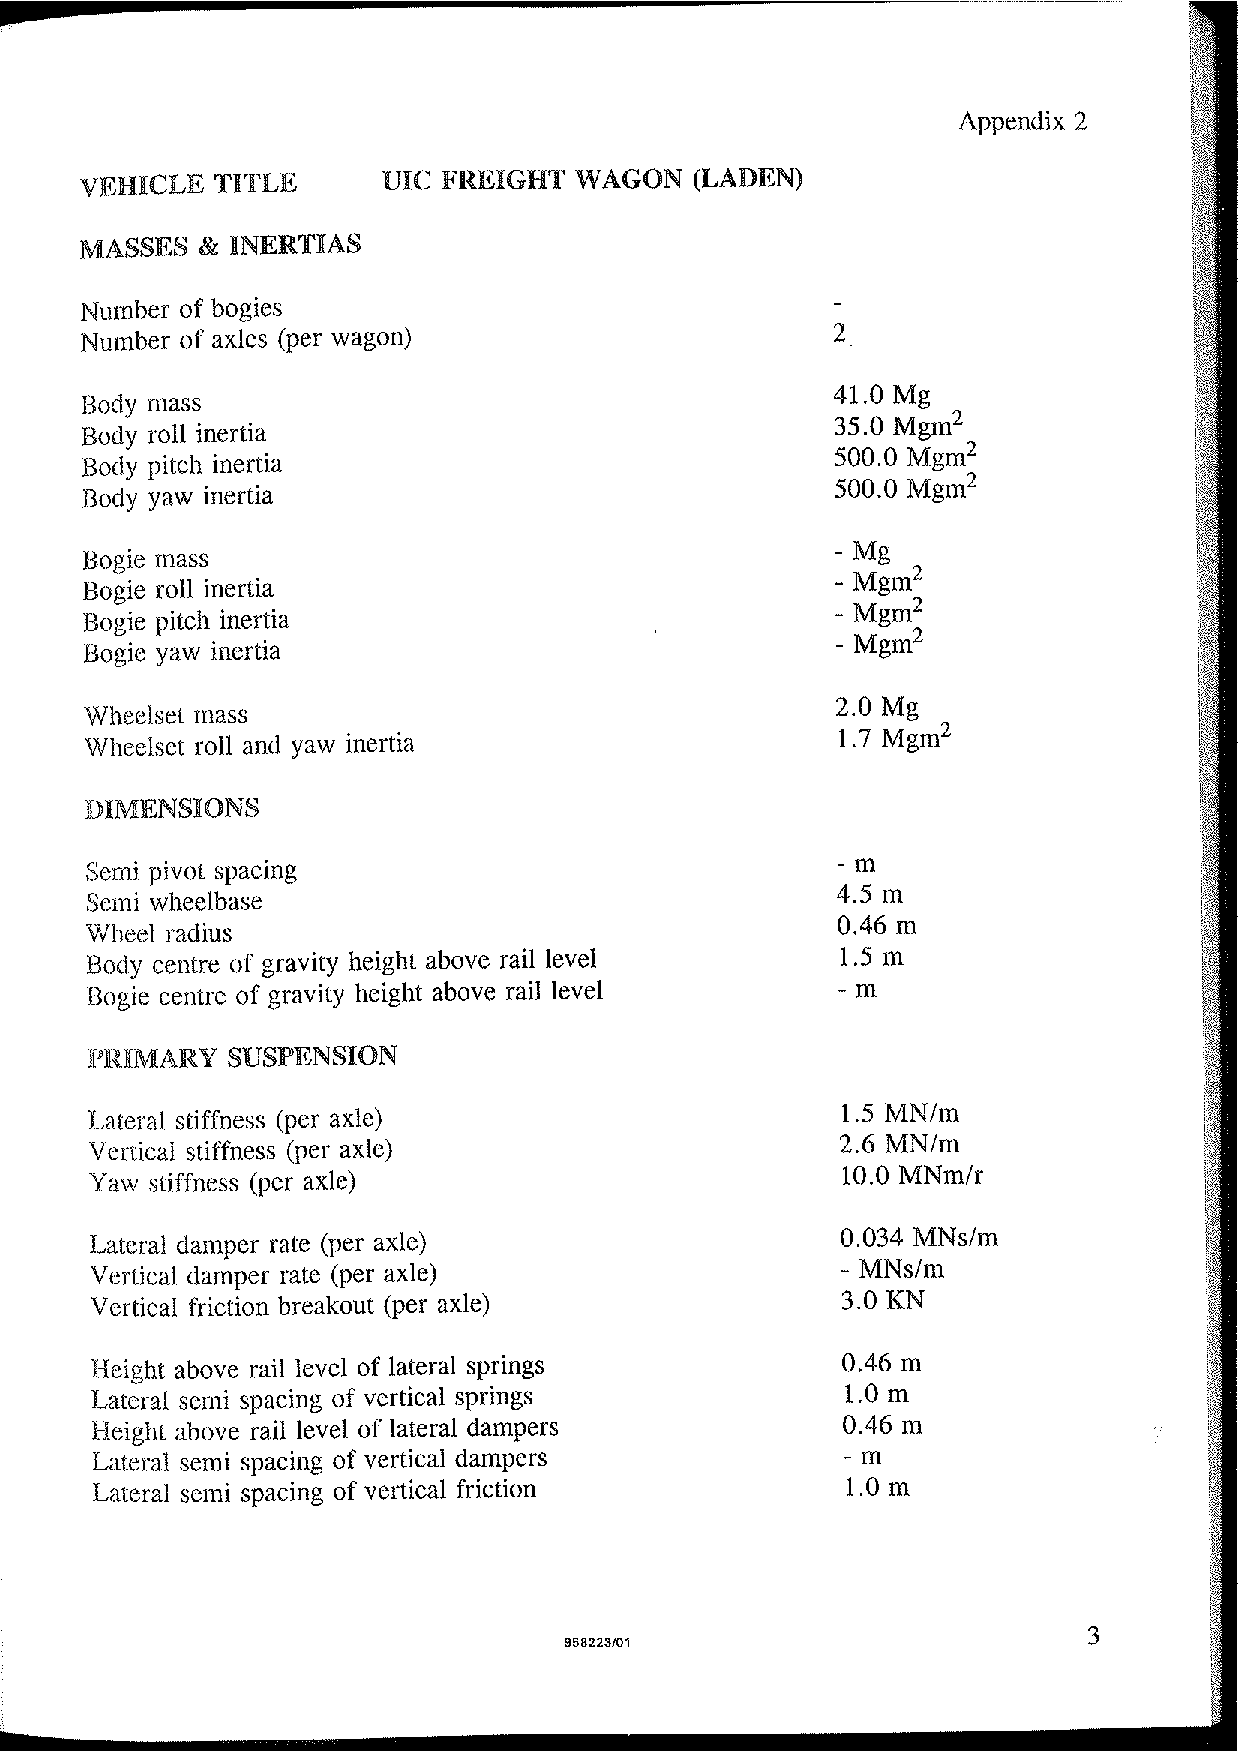
\includegraphics[width=\textwidth]{vp21}
    \caption{UIC FREIGHT WAGON (LADEN). Extract from \cite[Appendix 2]{d181dt329}}
\end{figure}

\begin{figure}[h]
    \centering
    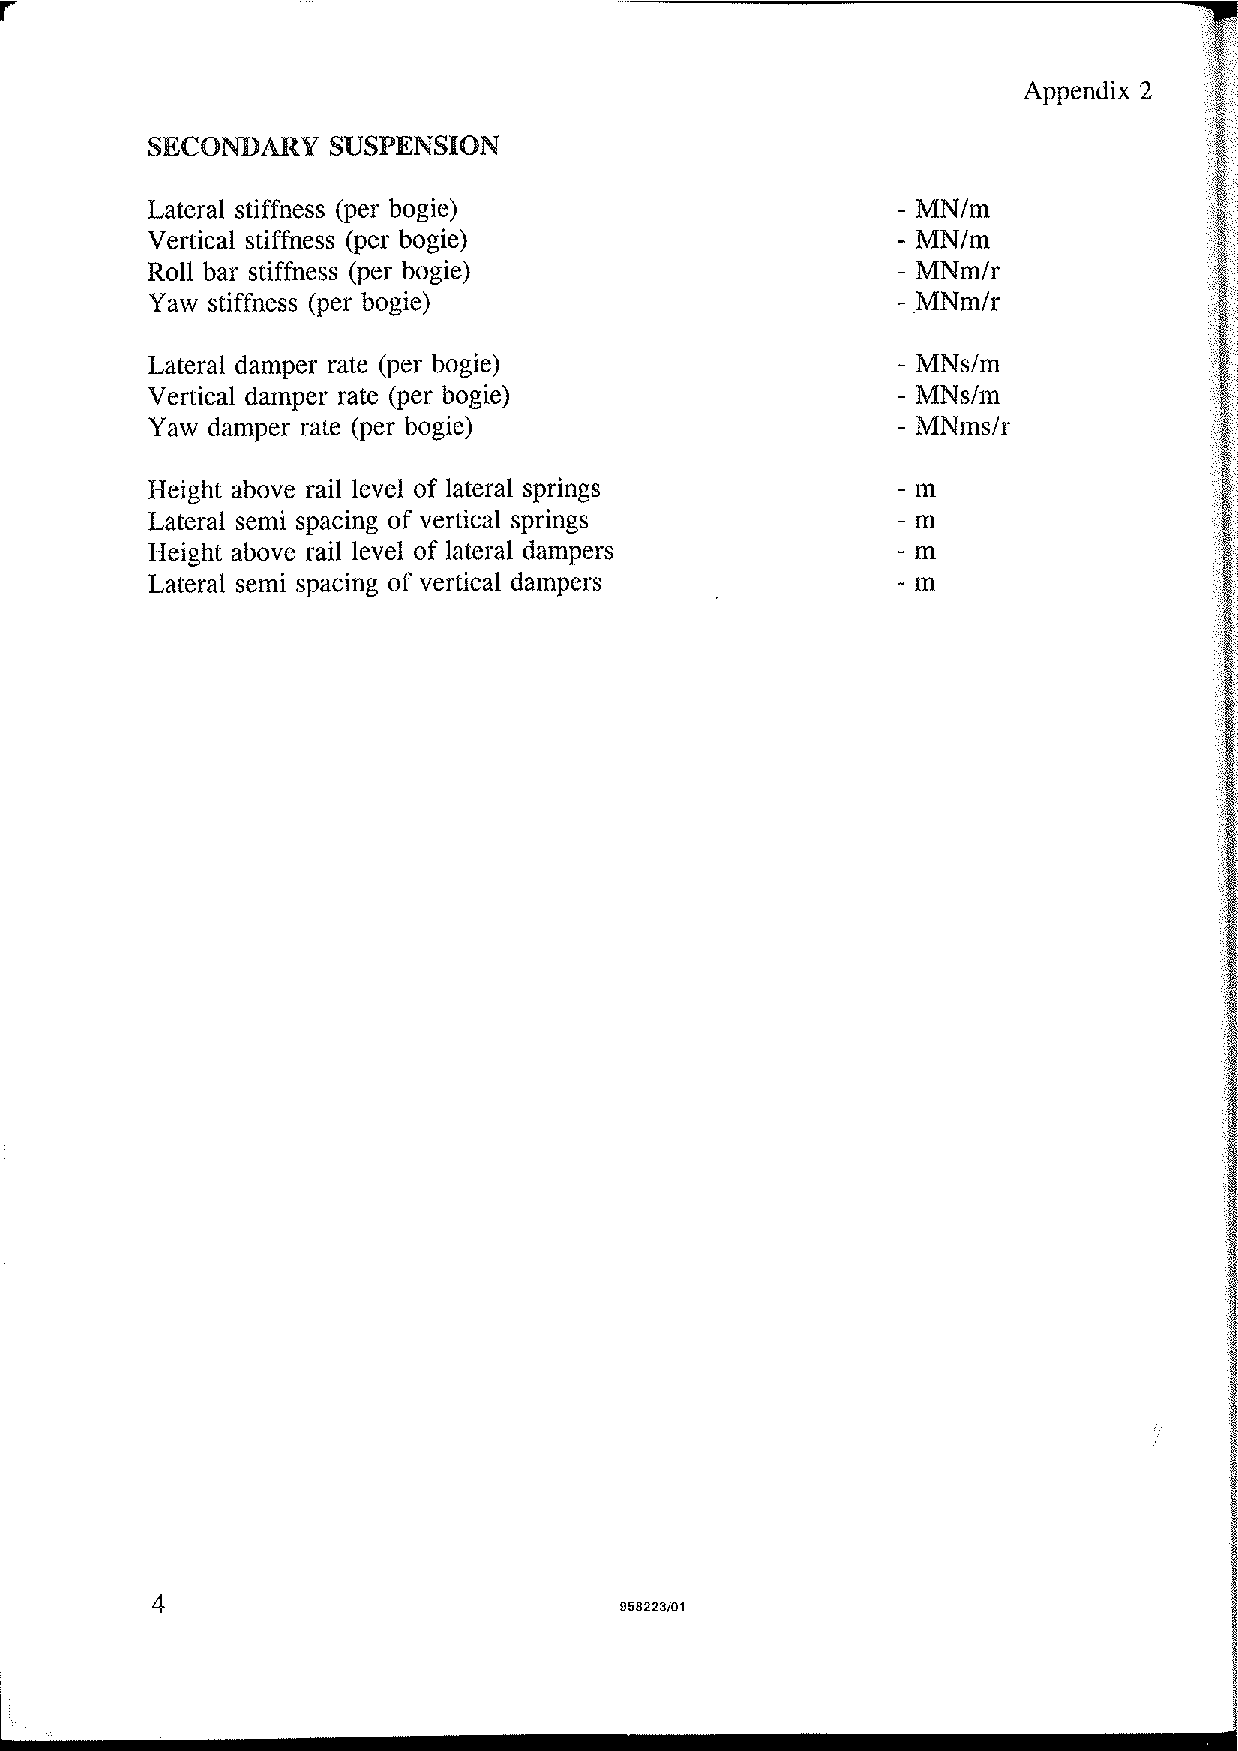
\includegraphics[width=\textwidth]{vp22}
    \caption{UIC FREIGHT WAGON (LADEN). Extract from \cite[Appendix 2]{d181dt329}}
\end{figure}

\begin{figure}[h]
    \centering
    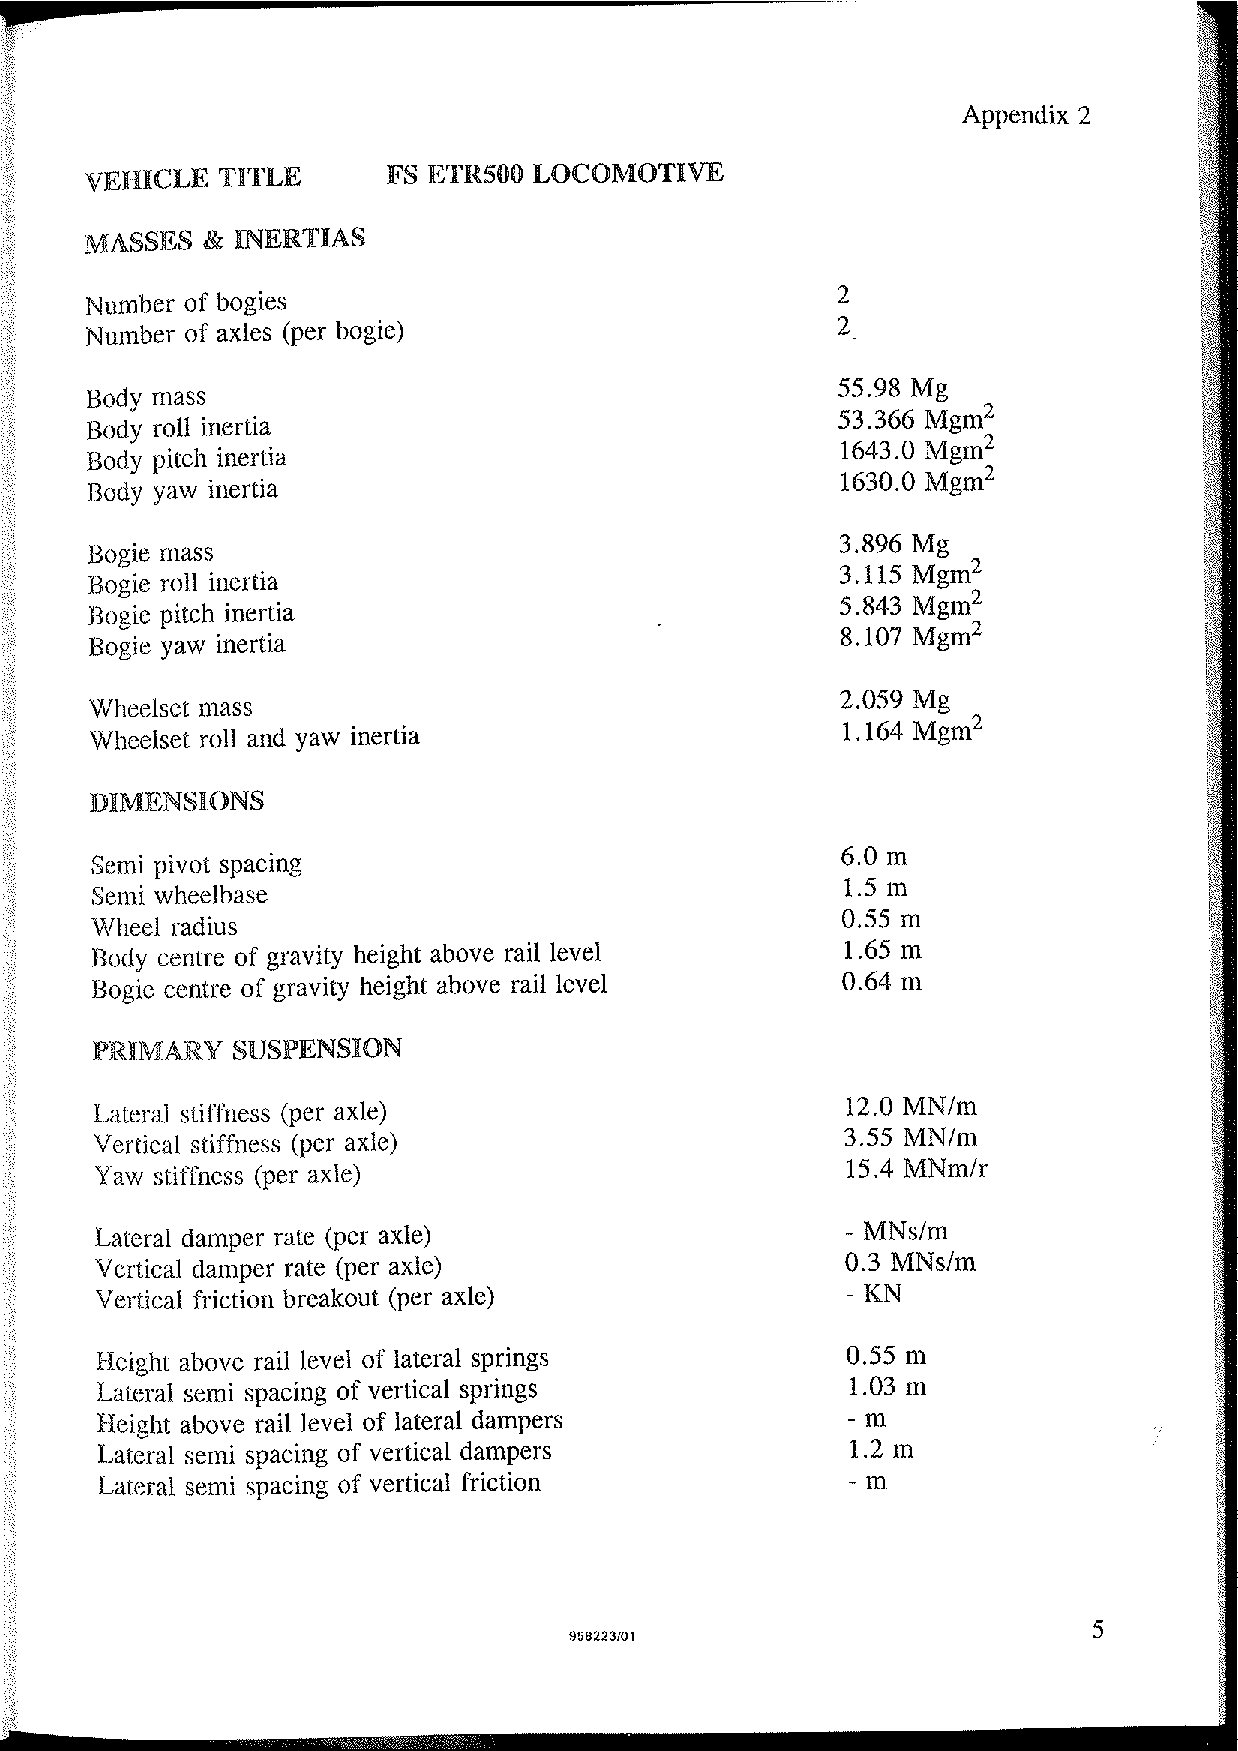
\includegraphics[width=\textwidth]{vp31}
    \caption{FS ETR500 LOCOMOTIVE. Extract from \cite[Appendix 2]{d181dt329}}
\end{figure}

\begin{figure}[h]
    \centering
    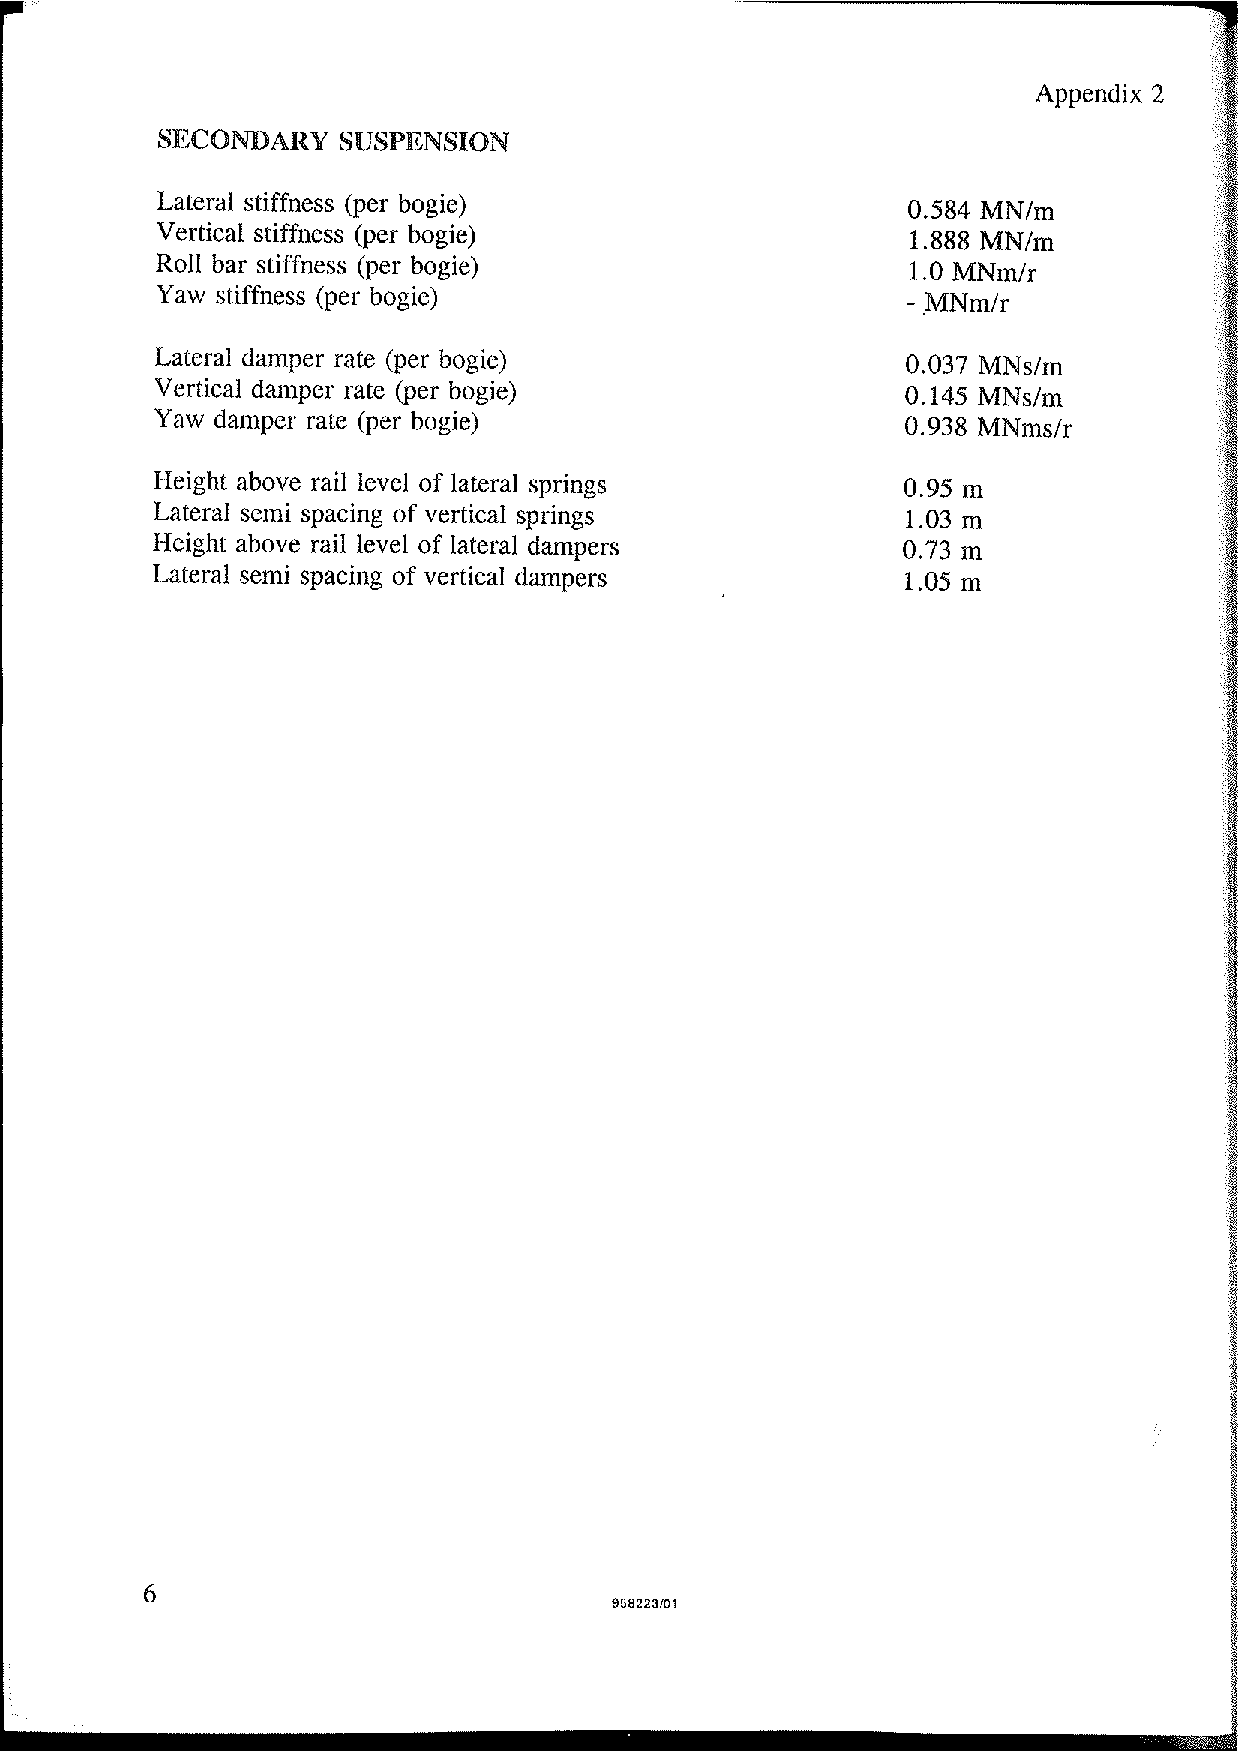
\includegraphics[width=\textwidth]{vp32}
    \caption{FS ETR500 LOCOMOTIVE. Extract from \cite[Appendix 2]{d181dt329}}
\end{figure}

\begin{figure}[h]
    \centering
    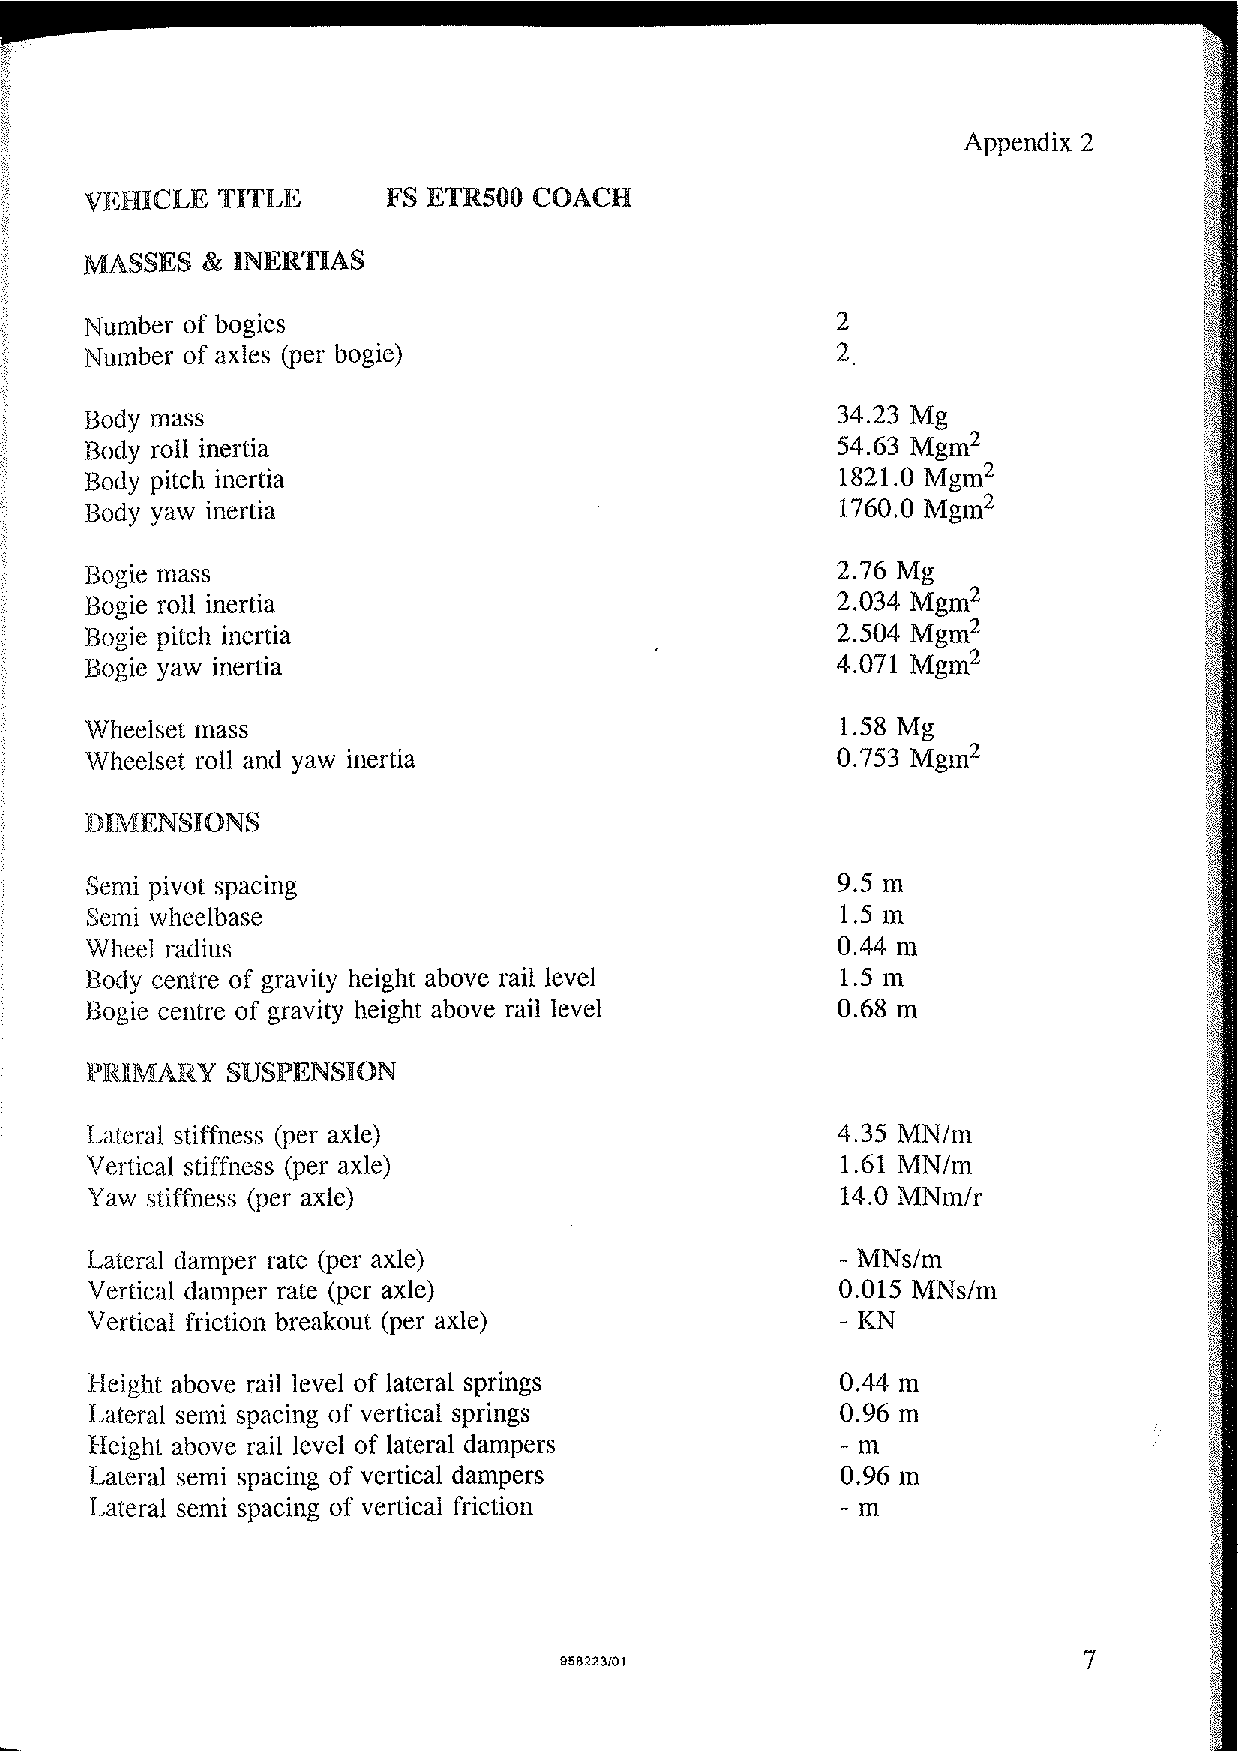
\includegraphics[width=\textwidth]{vp41}
    \caption{FS ETR500 COACH. Extract from \cite[Appendix 2]{d181dt329}}
\end{figure}

\begin{figure}[h]
    \centering
    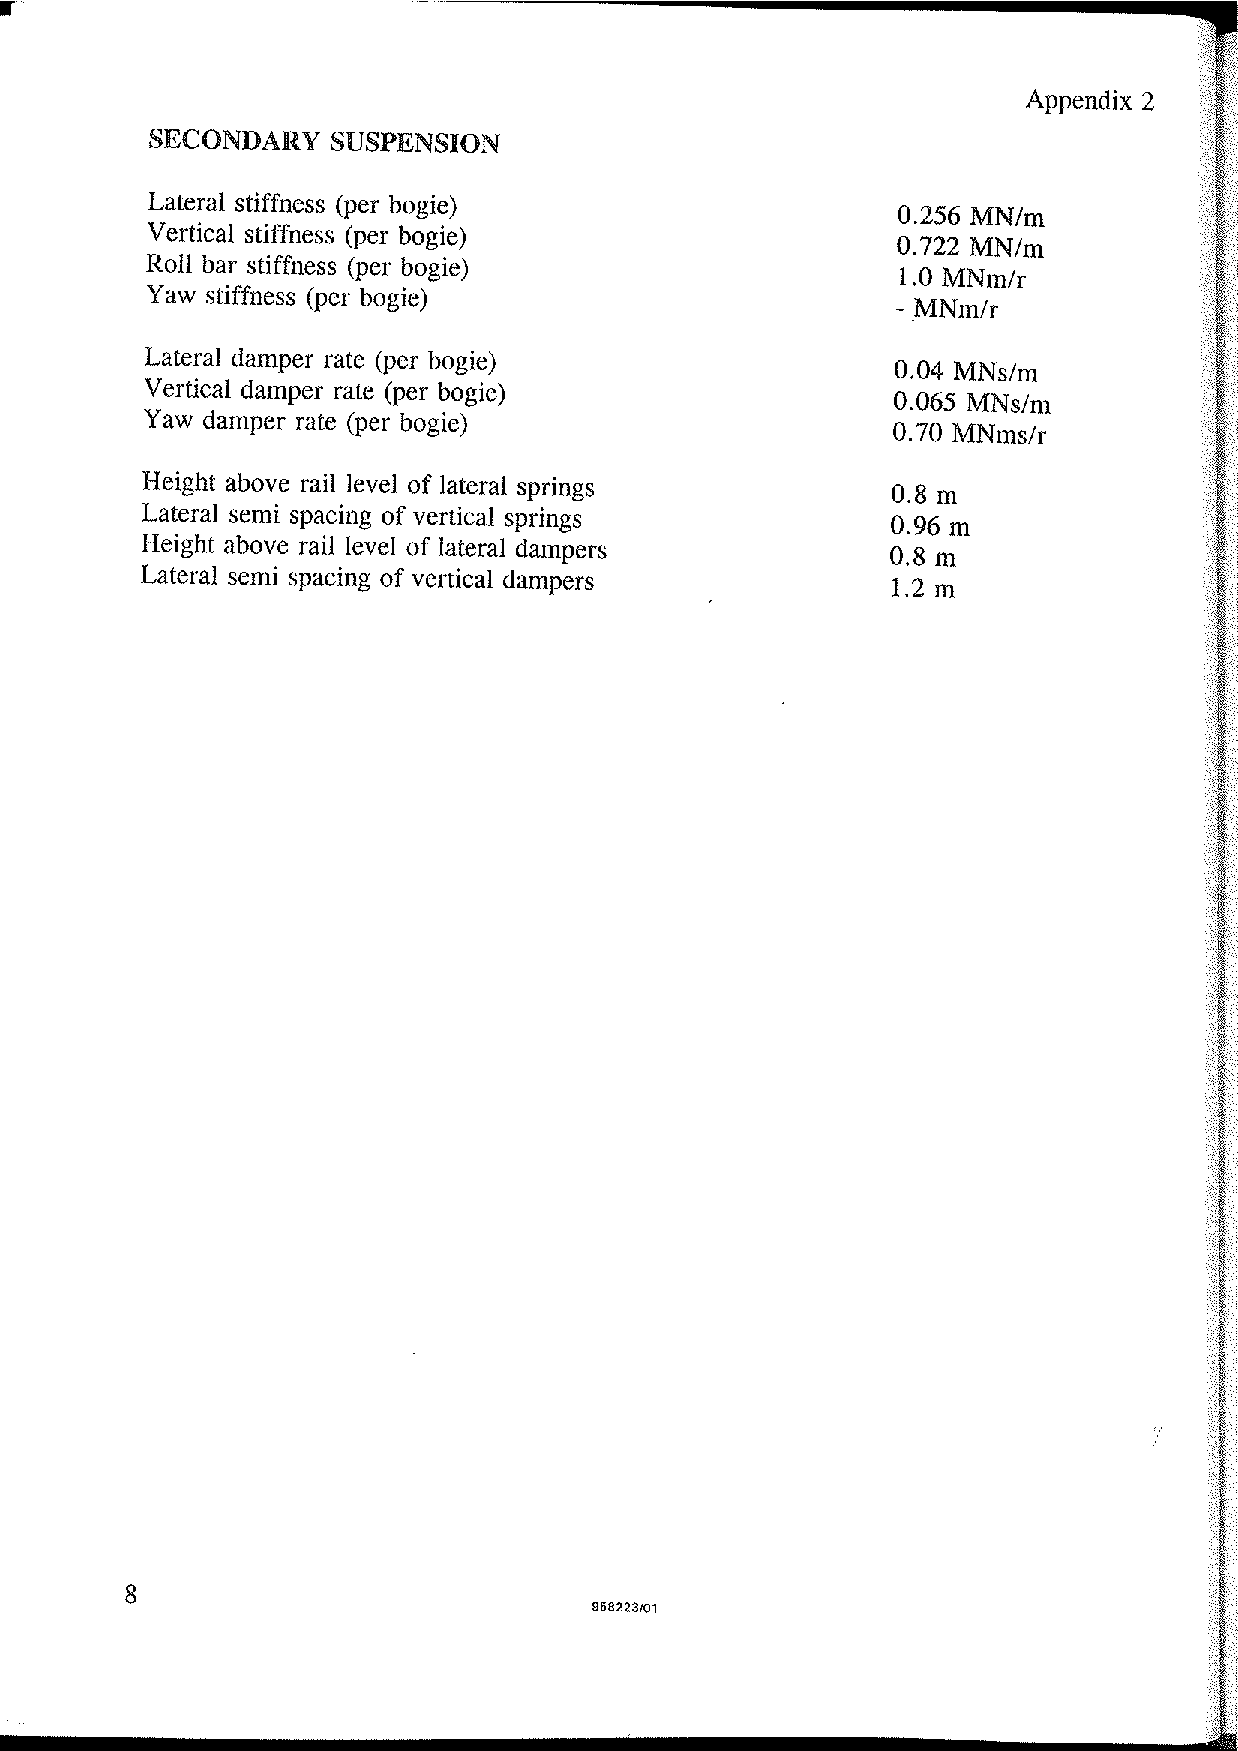
\includegraphics[width=\textwidth]{vp42}
    \caption{FS ETR500 COACH. Extract from \cite[Appendix 2]{d181dt329}}
\end{figure}

\begin{figure}[h]
    \centering
    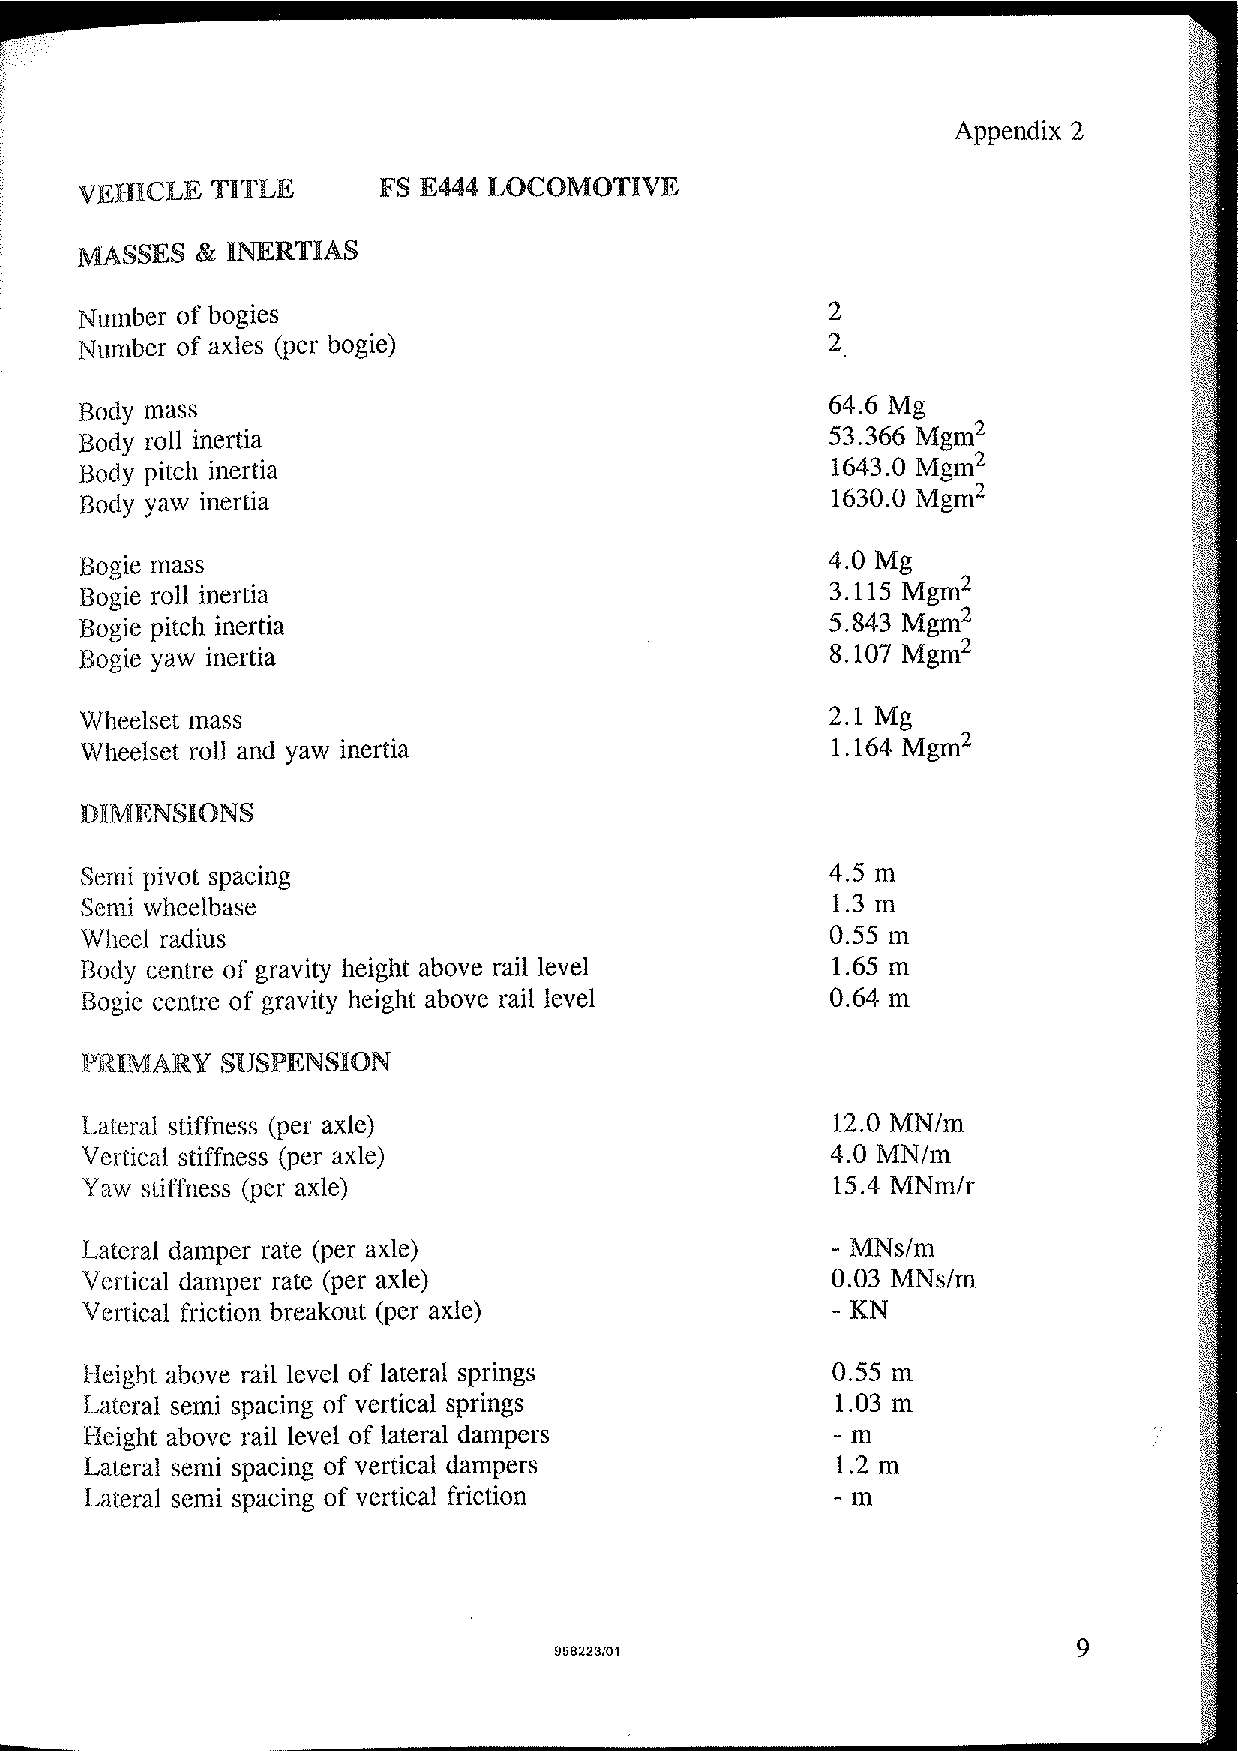
\includegraphics[width=\textwidth]{vp51}
    \caption{FS E444 LOCOMOTIVE. Extract from \cite[Appendix 2]{d181dt329}}
\end{figure}

\begin{figure}[h]
    \centering
    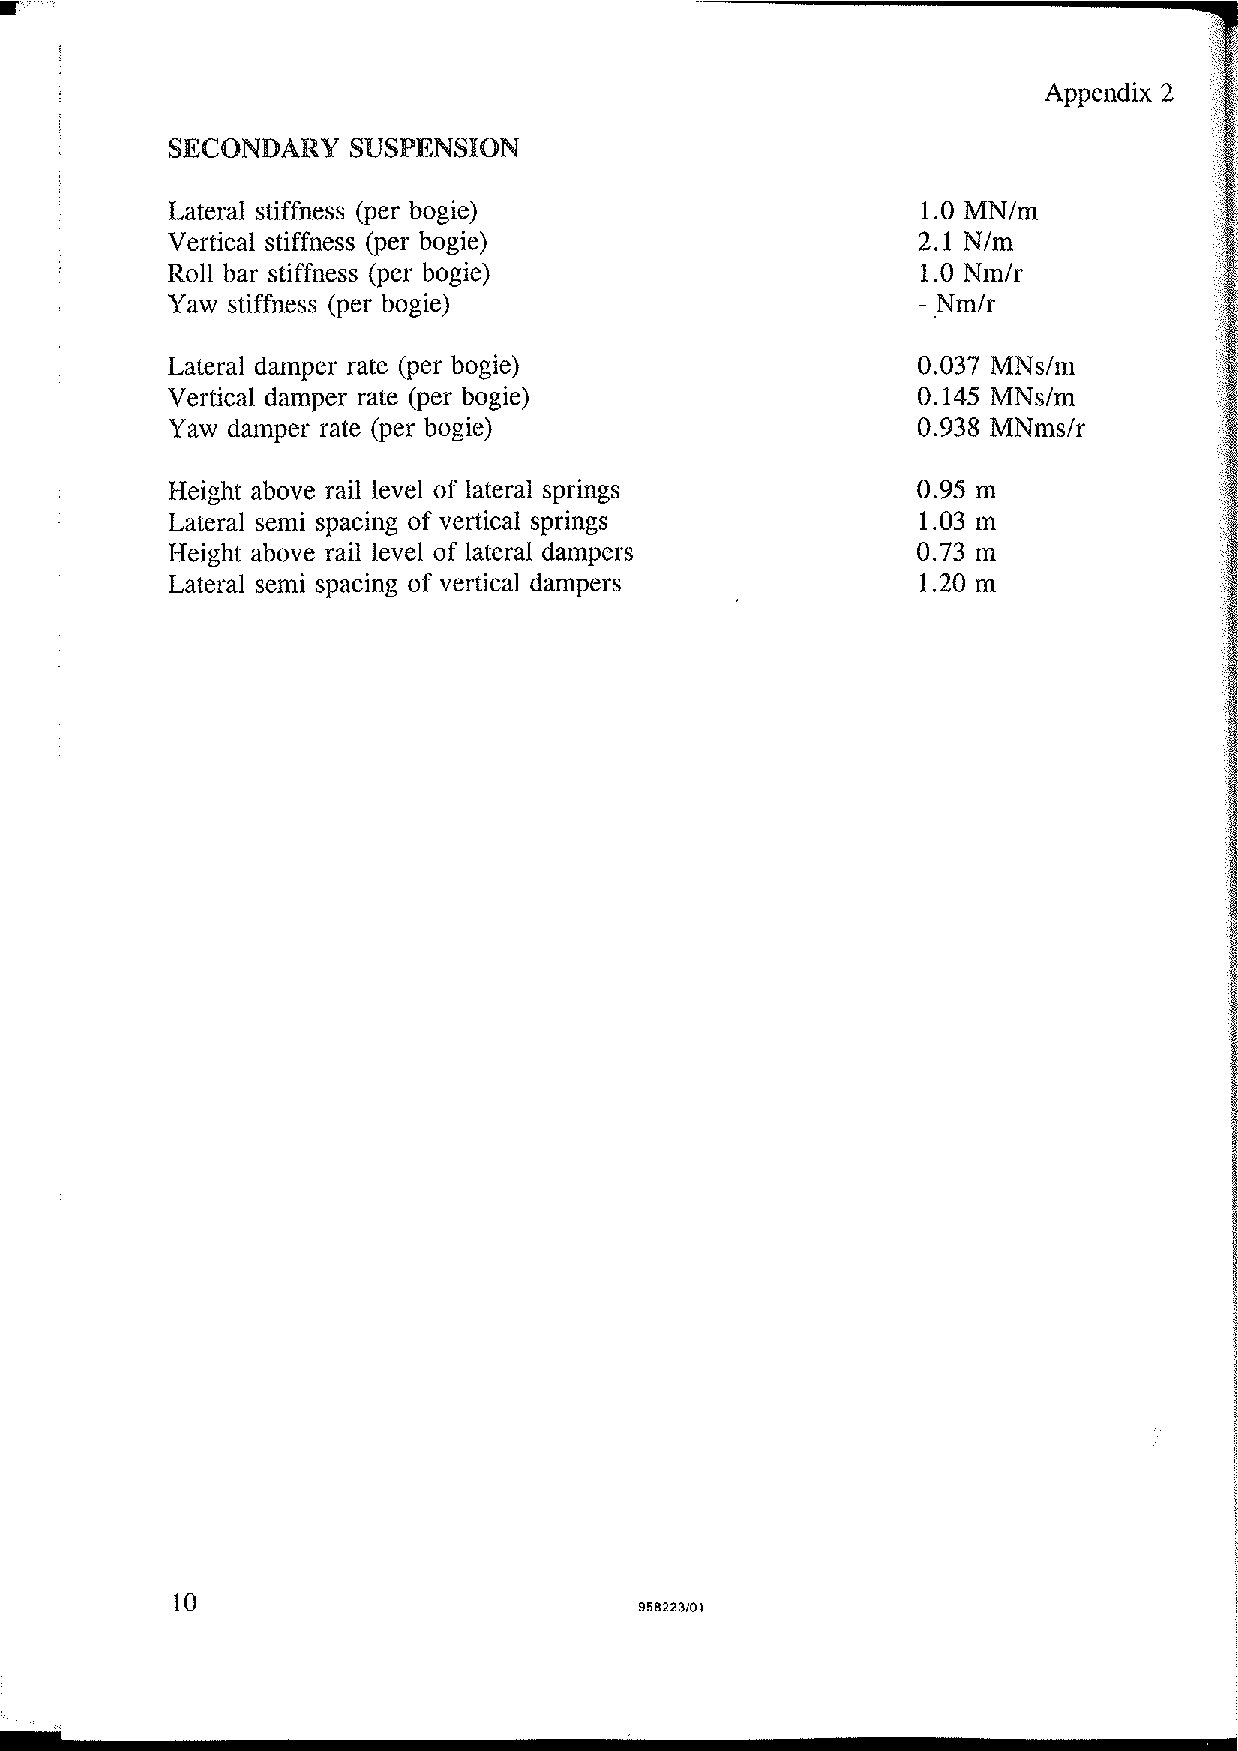
\includegraphics[width=\textwidth]{vp52}
    \caption{FS E444 LOCOMOTIVE. Extract from \cite[Appendix 2]{d181dt329}}
\end{figure}

\begin{figure}[h]
    \centering
    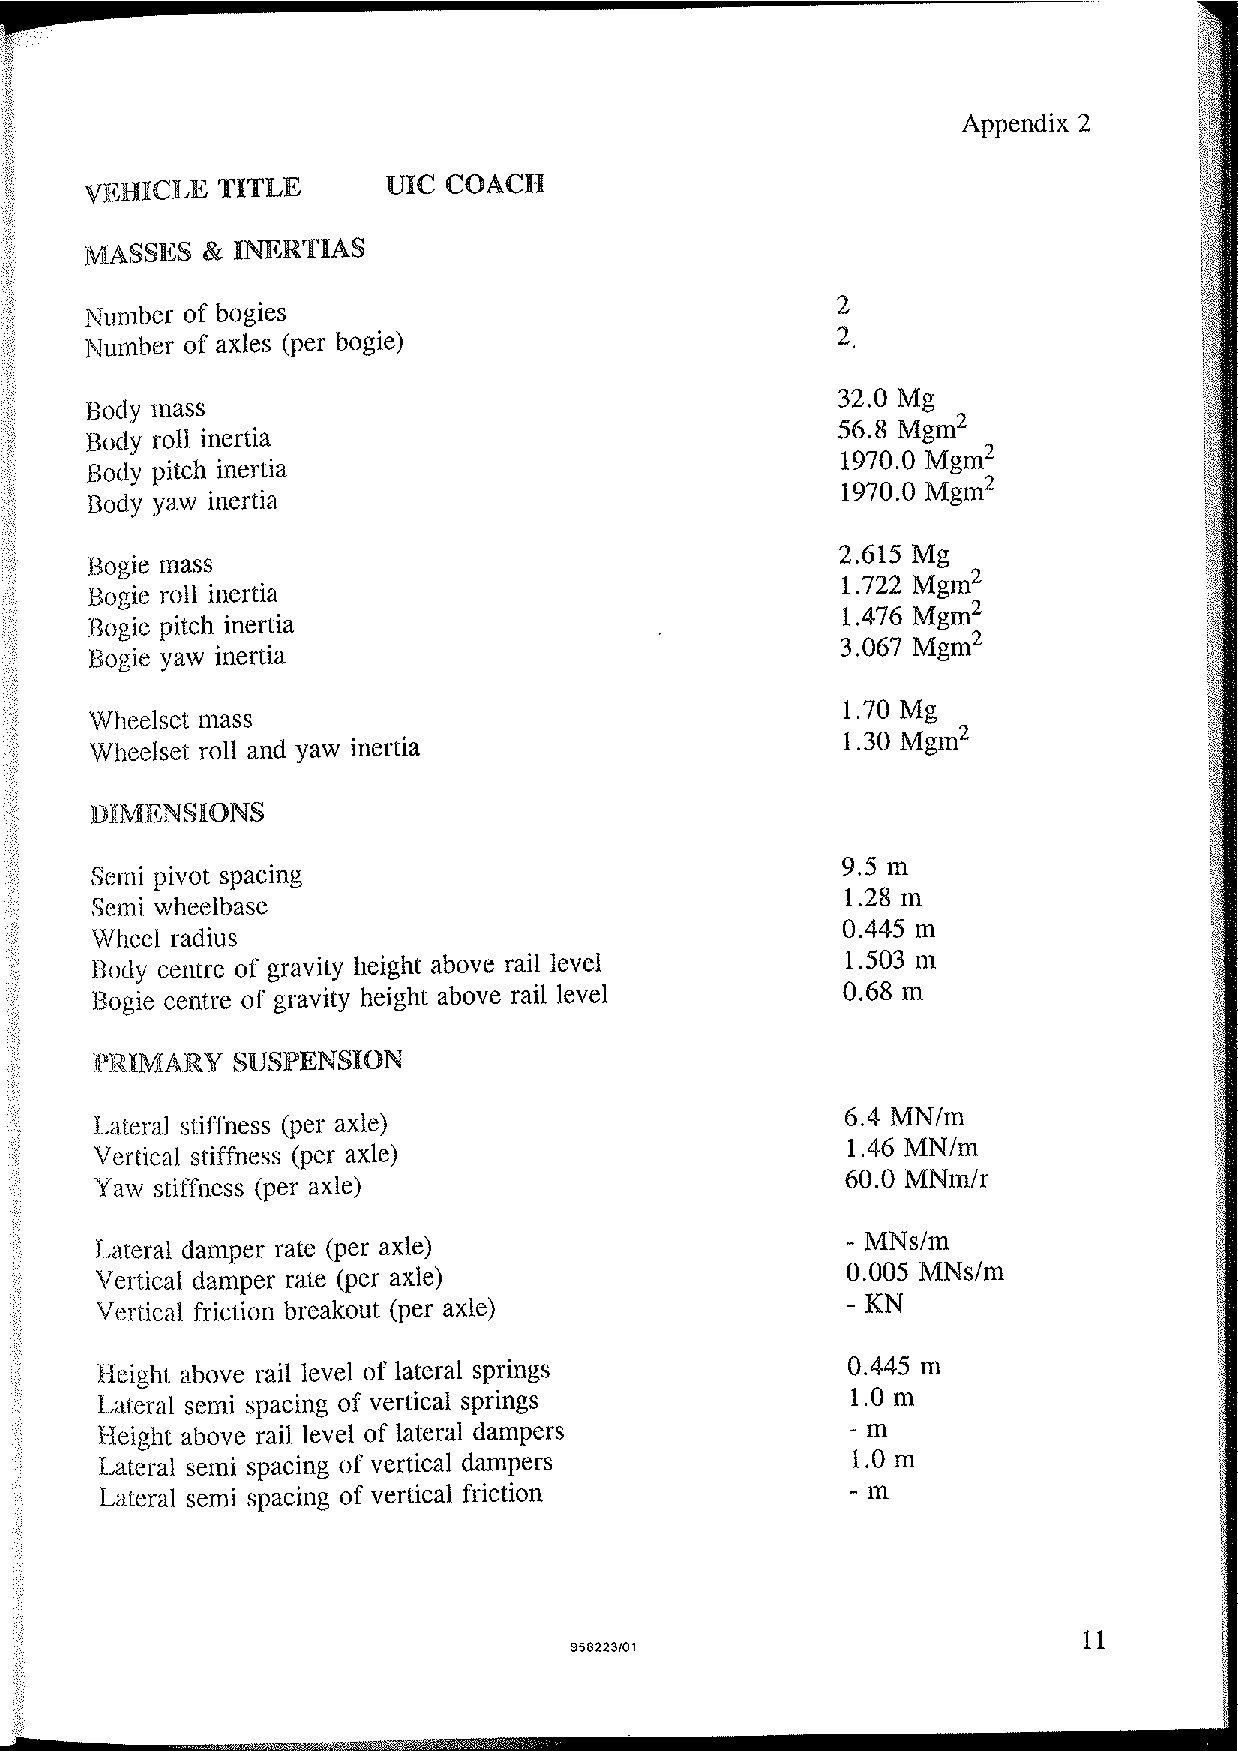
\includegraphics[width=\textwidth]{vp61}
    \caption{UIC COACH. Extract from \cite[Appendix 2]{d181dt329}}
\end{figure}

\begin{figure}[h]
    \centering
    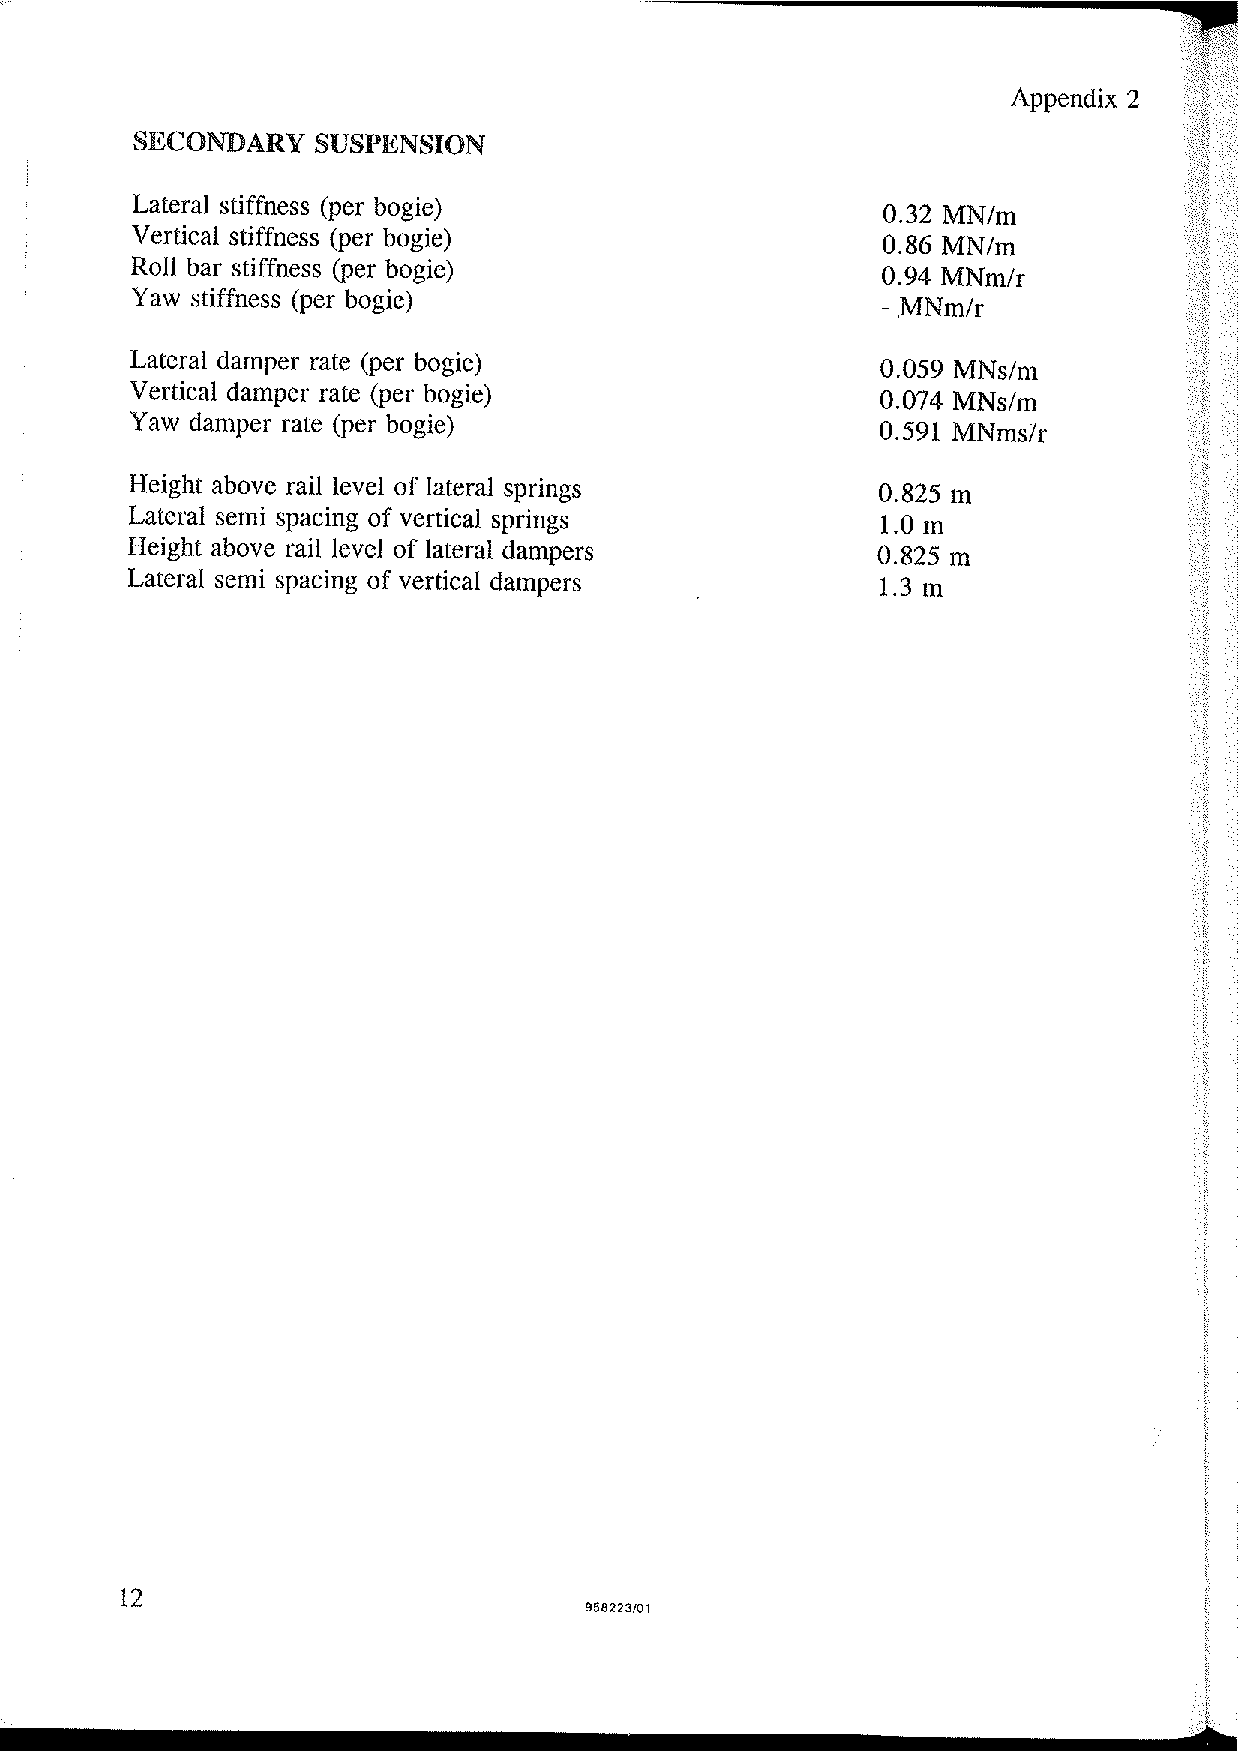
\includegraphics[width=\textwidth]{vp62}
    \caption{UIC COACH. Extract from \cite[Appendix 2]{d181dt329}}
\end{figure}

\begin{figure}[h]    \centering
    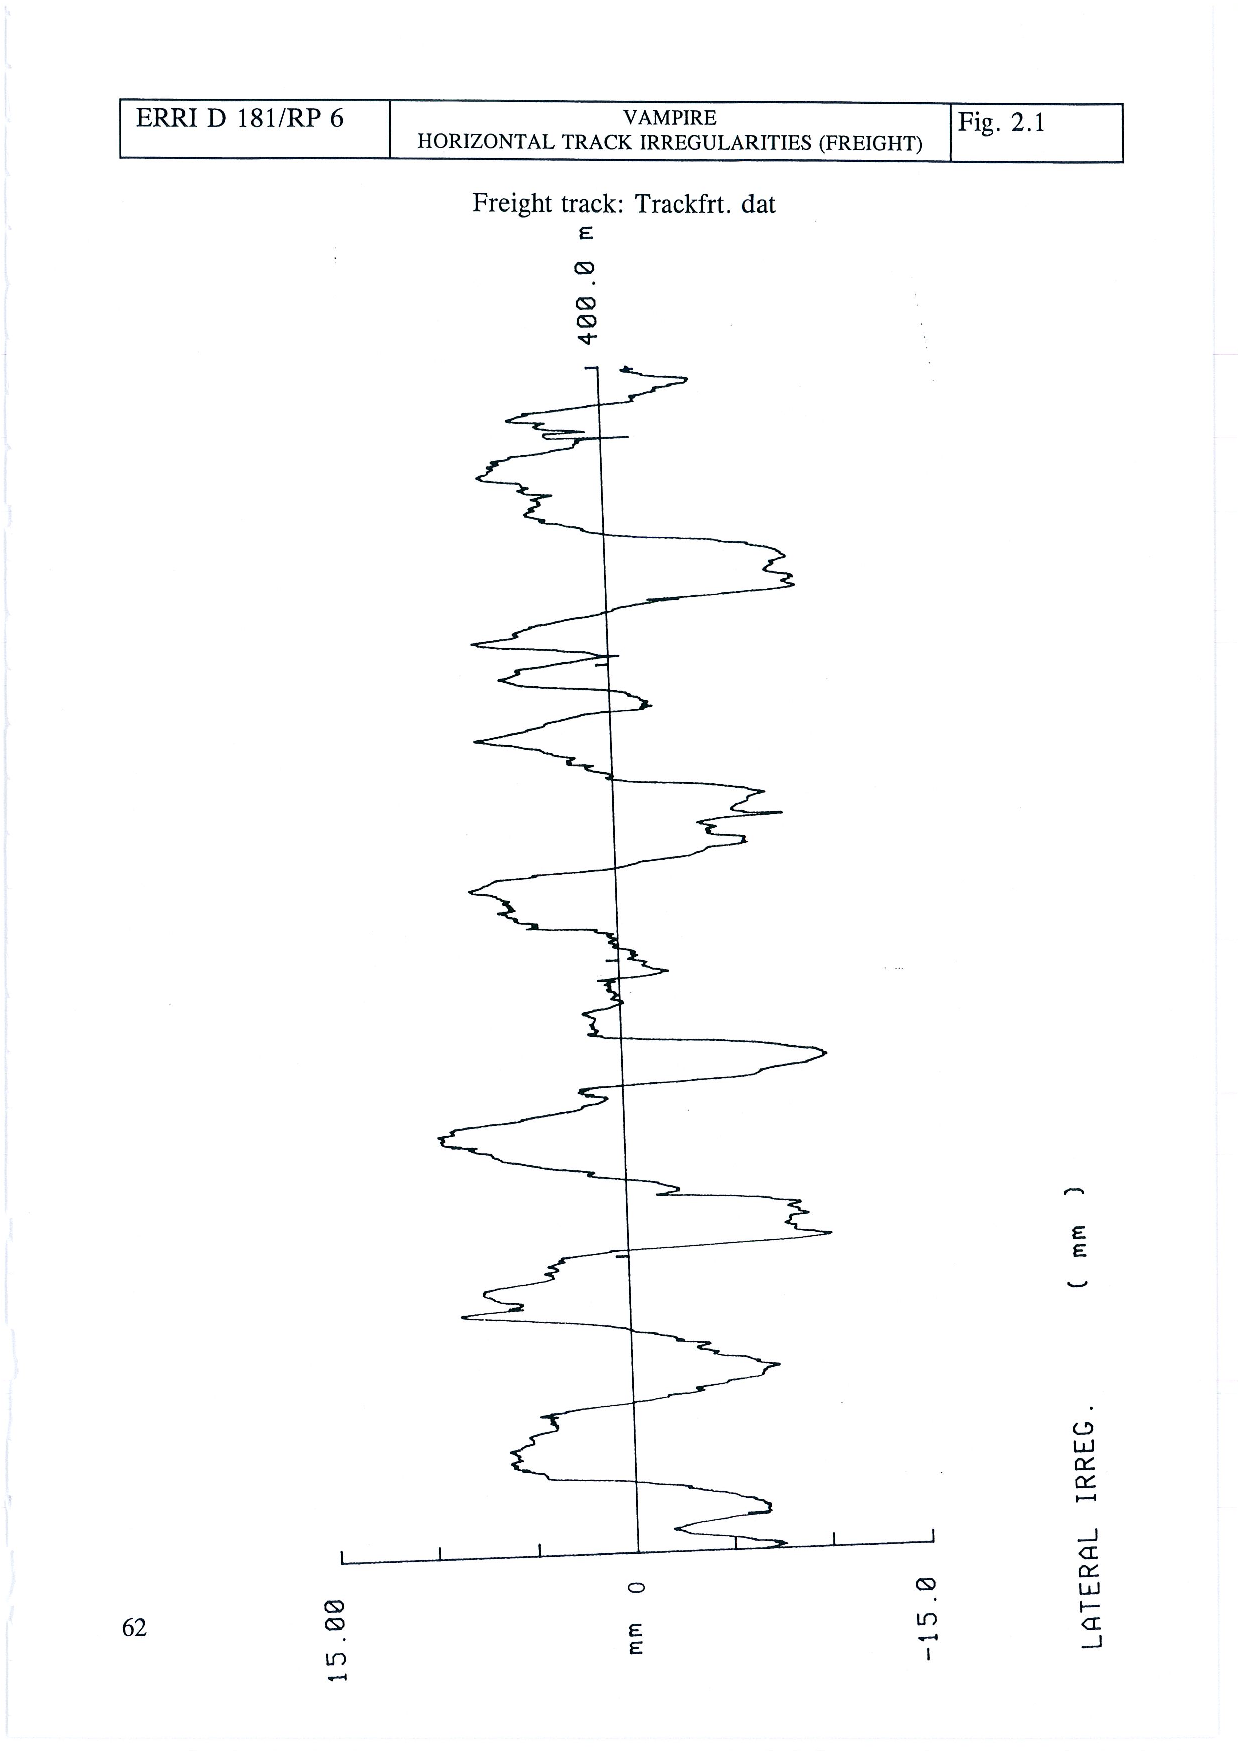
\includegraphics[width=\textwidth]{track1}
    \caption{Horizontal track irregularities for freight trains. Extract from \cite[Figure 2.1]{d181}}
    \label{fig:track1}
\end{figure}

\begin{figure}[h]
    \centering
    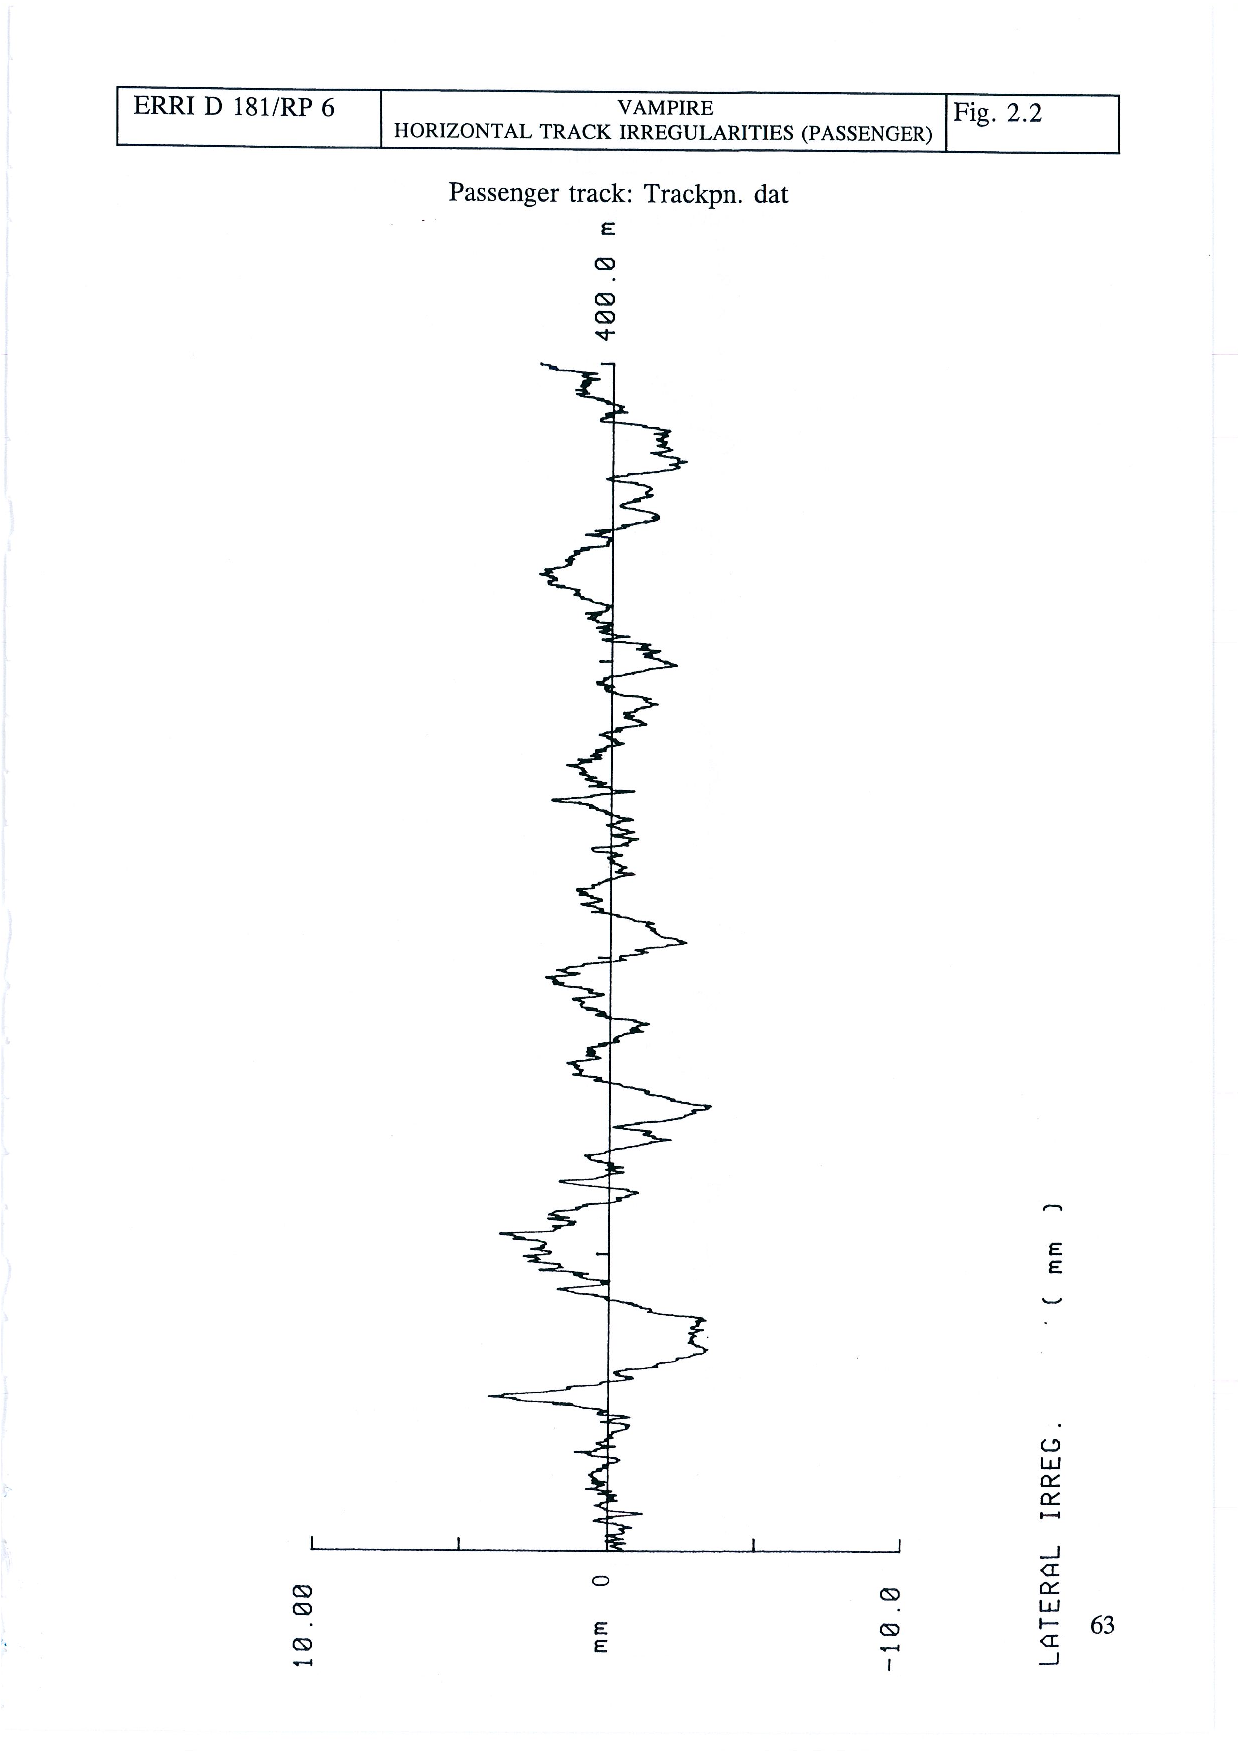
\includegraphics[width=\textwidth]{track2}
    \caption{Horizontal track irregularities for standard passenger trains. Extract from \cite[Figure 2.1]{d181}}
\end{figure}

\begin{figure}[h]
    \centering
    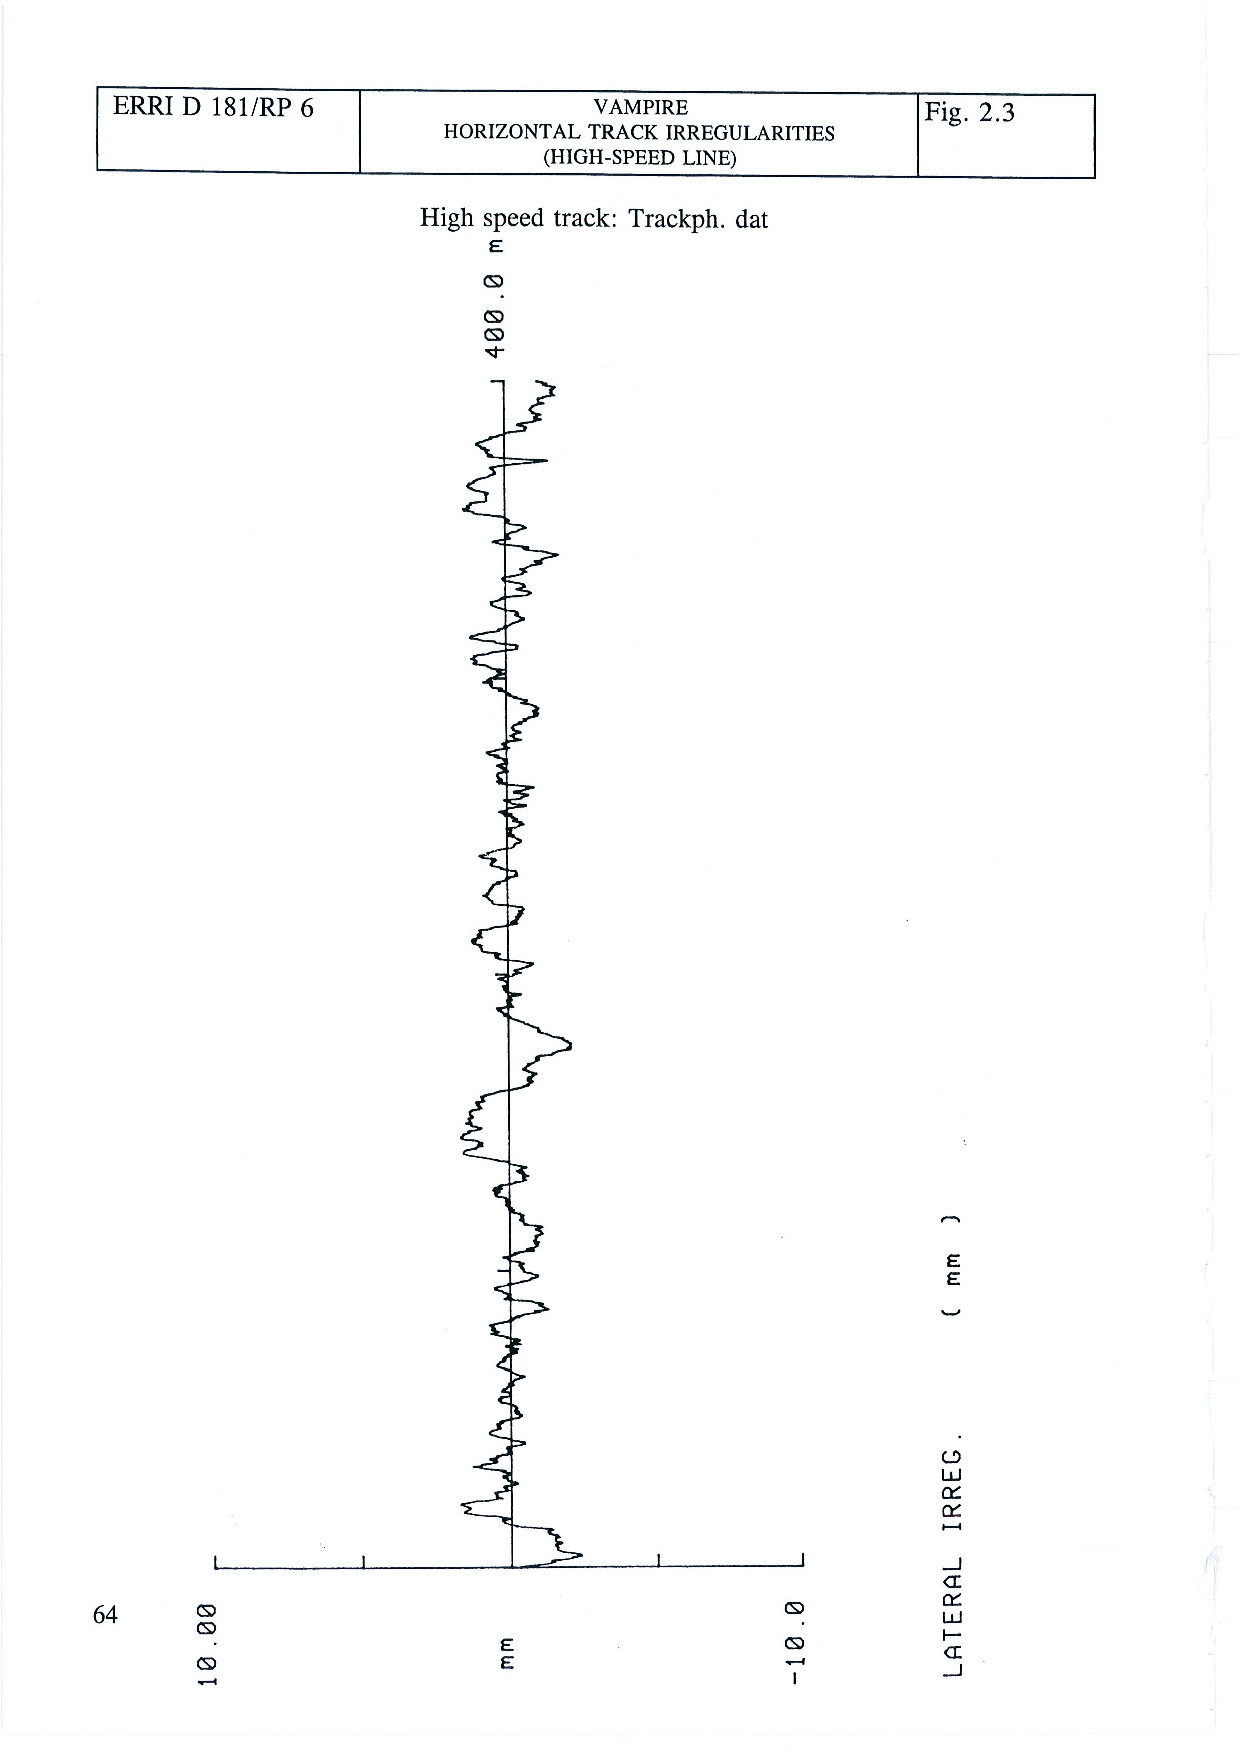
\includegraphics[width=\textwidth]{track3}
    \caption{Horizontal track irregularities for high speed passenger train. Extract from \cite[Figure 2.1]{d181}}
    \label{fig:track3}
\end{figure}

\begin{table}[h]
    \centering
    \begin{tabular}{c|c|c|c}
    \hline
    \multirow{2}{*}{Freight train: Principle axle repeat patterns} & dist & \multicolumn{2}{c}{Speed} \\
    & m & 60 km/h & 100 km/h \\
    \hline
    wagon n axle 2 - wagon n+1 axle 1 & 4.00 & 4.17 & 6.94 \\
    wagon wheelbase & 9.00 & 1.85 & 3.09 \\
    wagon n axle m - wagon n+1 axle m & 13.0 & 1.28 & 2.14 \\
    wagon n axle m - wagon n+2 axle m & 26.0 & 0.64 & 1.07 \\
    \hline
    \multirow{2}{*}{Passenger train: Principle axle repeat patterns} & dist & \multicolumn{2}{c}{Speed} \\
    & m & 160 km/h & 200 km/h \\
    \hline
    coach n axle 1 - 2, and coach n axle 3 - 4 & 2.56 & 17.36 & 21.70 \\
    coach n axle m - coach n+1 axle m & 26.4 & 1.68 & 2.10 \\
    coach n axle m - coach n+2 axle m & 52.8 & 0.84 & 1.05 \\
    \hline
    \multirow{2}{*}{ETR 500 train: Principle axle repeat patterns} & dist & \multicolumn{2}{c}{Speed} \\
    & m & 300 km/h & 350 km/h \\
    \hline
    coach n axle 1 - 2 and coach n axle 3 - 4 & 3.0 & 27.78 & 32.41 \\
    coach n axle m - coach n+1 axle m & 26.1 & 3.19 & 3.72 \\
    coach n axle m - coach n+2 axle m & 52.2 & 1.60 & 1.86 \\
    coach n axle m - coach n+3 axle m & 69.3 & 1.20 & 1.40 \\
    \hline
    \end{tabular}
    \caption{Axle repeat patterns and typical frequencies. Extracted from \cite[Appendix C]{d181dt329}}
    \label{tab:329axlerepeat}
\end{table}

\begin{table}[h]
    \centering
    \begin{tabular}{c|c|c|c}
    \hline
    Kinematic wavelength, m & Freight train & Passenger train & ETR500 train \\
    \hline
    Locomotive & 39 - 45 & 32 - 38 & 39 - 45 \\
    Coach/wagon & 24 - 39 & 34 - 38 & 36 - 40 \\
    \hline
    \end{tabular}
    \caption{Kinematic wavelength ranges per vehicle, with BR P1 profiles. Extracted from \cite[Appendix C]{d181dt329}}
    \label{tab:329kinematicwavelength}
\end{table}

\chapter{Speeds which do not require dynamic compatibility checks} \label{app:speedsafe}

\begin{figure}[h]
    \centering
    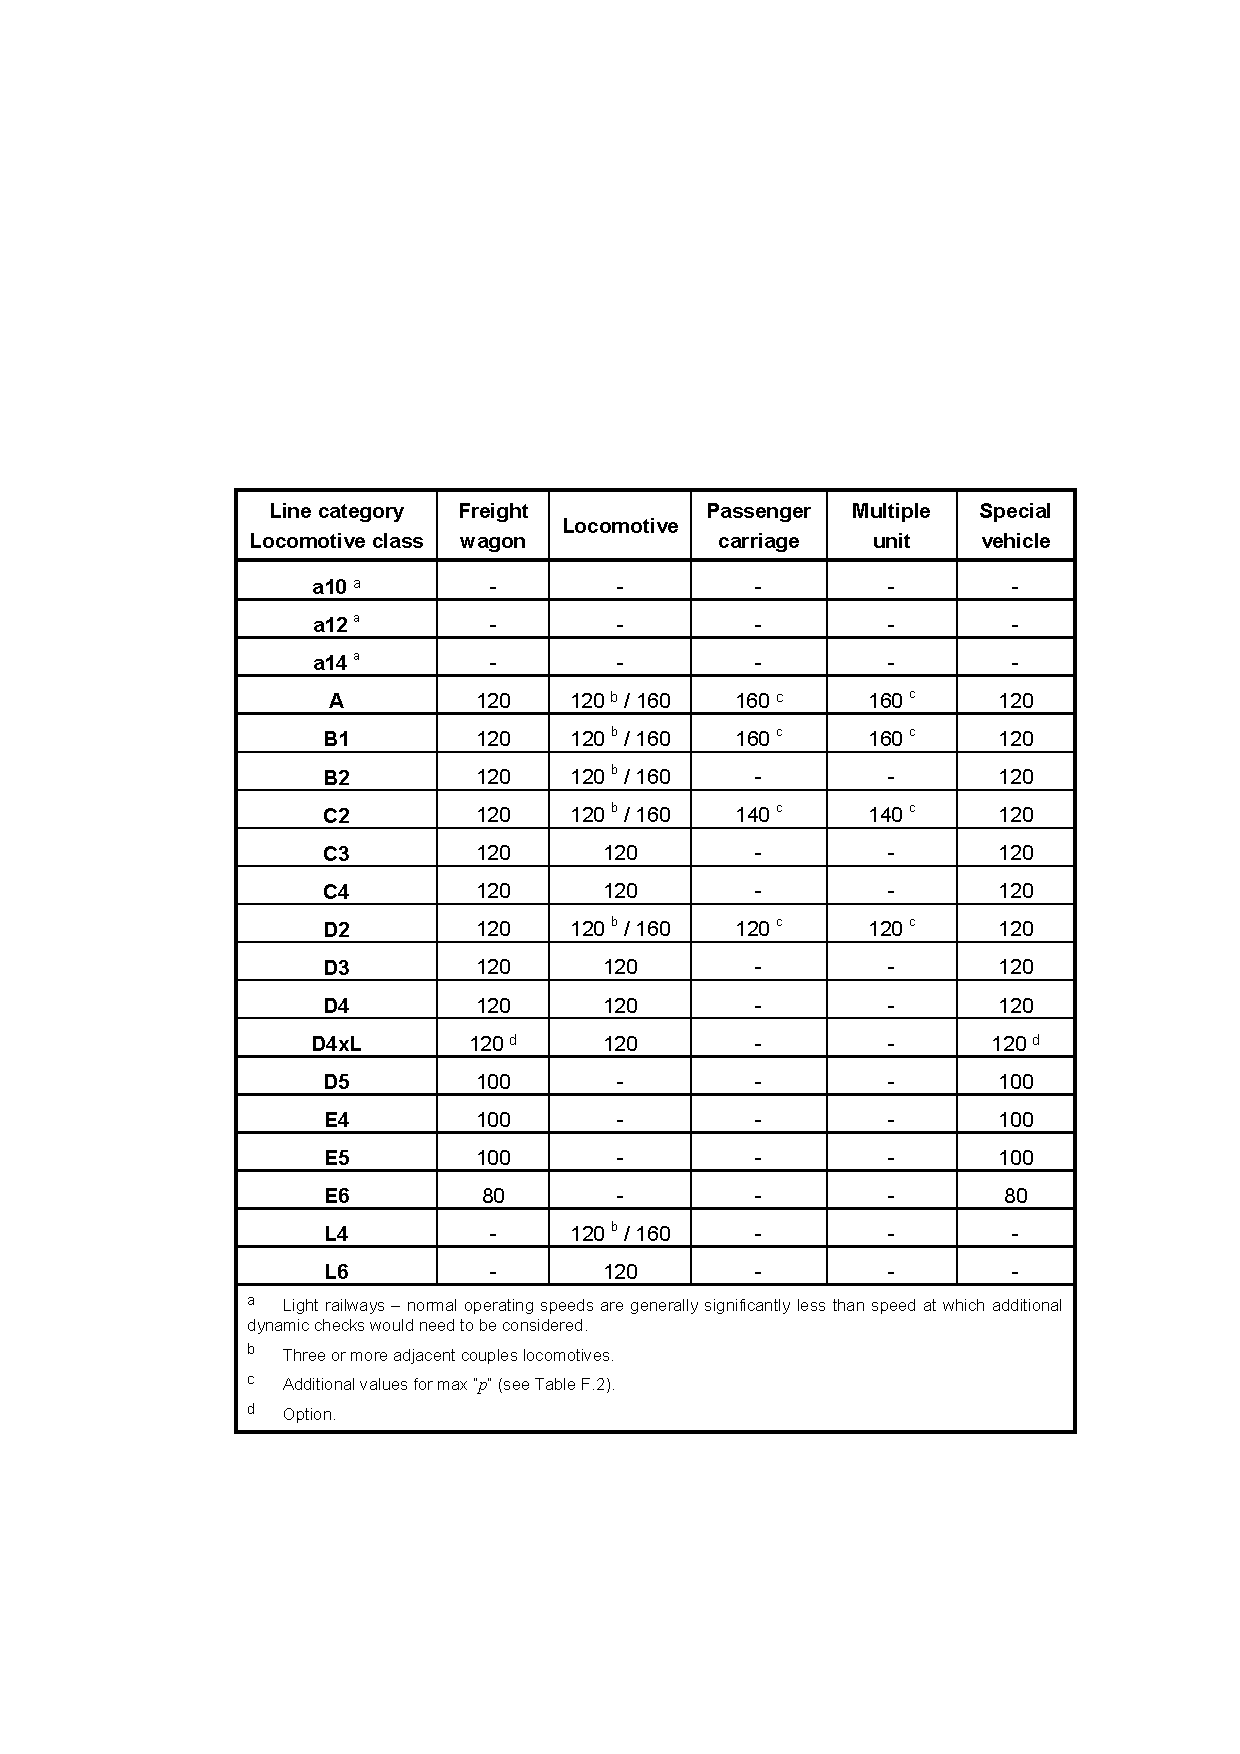
\includegraphics[width=0.7\textwidth]{speedsafe.pdf}
    \caption{Speed limit (in km/h) in relationship Line Category/Locomotive Class and vehicle type. Extract from \cite[Appendix F]{EC15528}}
\end{figure}

\chapter{MU-Groups and MU-Classes}\label{app:mu}

\section{Definition}
Multiple units can be grouped according to type of traffic service(high speed - long distance, intercity - regional and commuter/suburban) or to the kind of running gear (conventional bogies, articulated bogies and single axles).


In some cases due to potential excessive dynamic load effects in bridge line category checks are not sufficient to demonstrate compatibility. To minimise the need for undertaking a dynamic check of individual trains, several typical and wide spread MU-designs have been grouped in MU-classes. For these groups of vehicles, load models covering the specified design parameter ranges have been developed to allow the efficient dynamic analysis of bridges. For practical reasons, the number of MU classes was limited and for trains outside the range of parameters covered, the process of checking an individual train existing at the time of publication of this standard as state of the art shall be used.

Each MU-class is defined by:

\begin{enumerate}[-]
\item ranges of train parameters covered and;
\item a corresponding load model for carrying out dynamic checks on bridges.
\end{enumerate}

Each MU-Group comprises of serveral MU-Classes. Table

\begin{table}[h]
    \centering
    \begin{tabular}{c|c}
        \hline
        MU-Group & MU-Class\\
        \hline
        \multirow{2}{*}{conventional bogie(CB)} & $CB_1$ \\
        & $CB_2$ \\
        \hline
        \multirow{4}{*}{articulated bogie(AB)} & $AB_1$ \\
        & $AB_2$ \\
        & $AB_3$ \\
        & $AB_4$ \\
        \hline
        \multirow{2}{*}{single axle(SA)} & $SA_1$ \\
        & $SA_2$ \\
        \hline
    \end{tabular}
    \caption{Relationship MU-groups - MU-classes}
    \label{tab:MU}
\end{table} 

\begin{figure}[h]
\centering
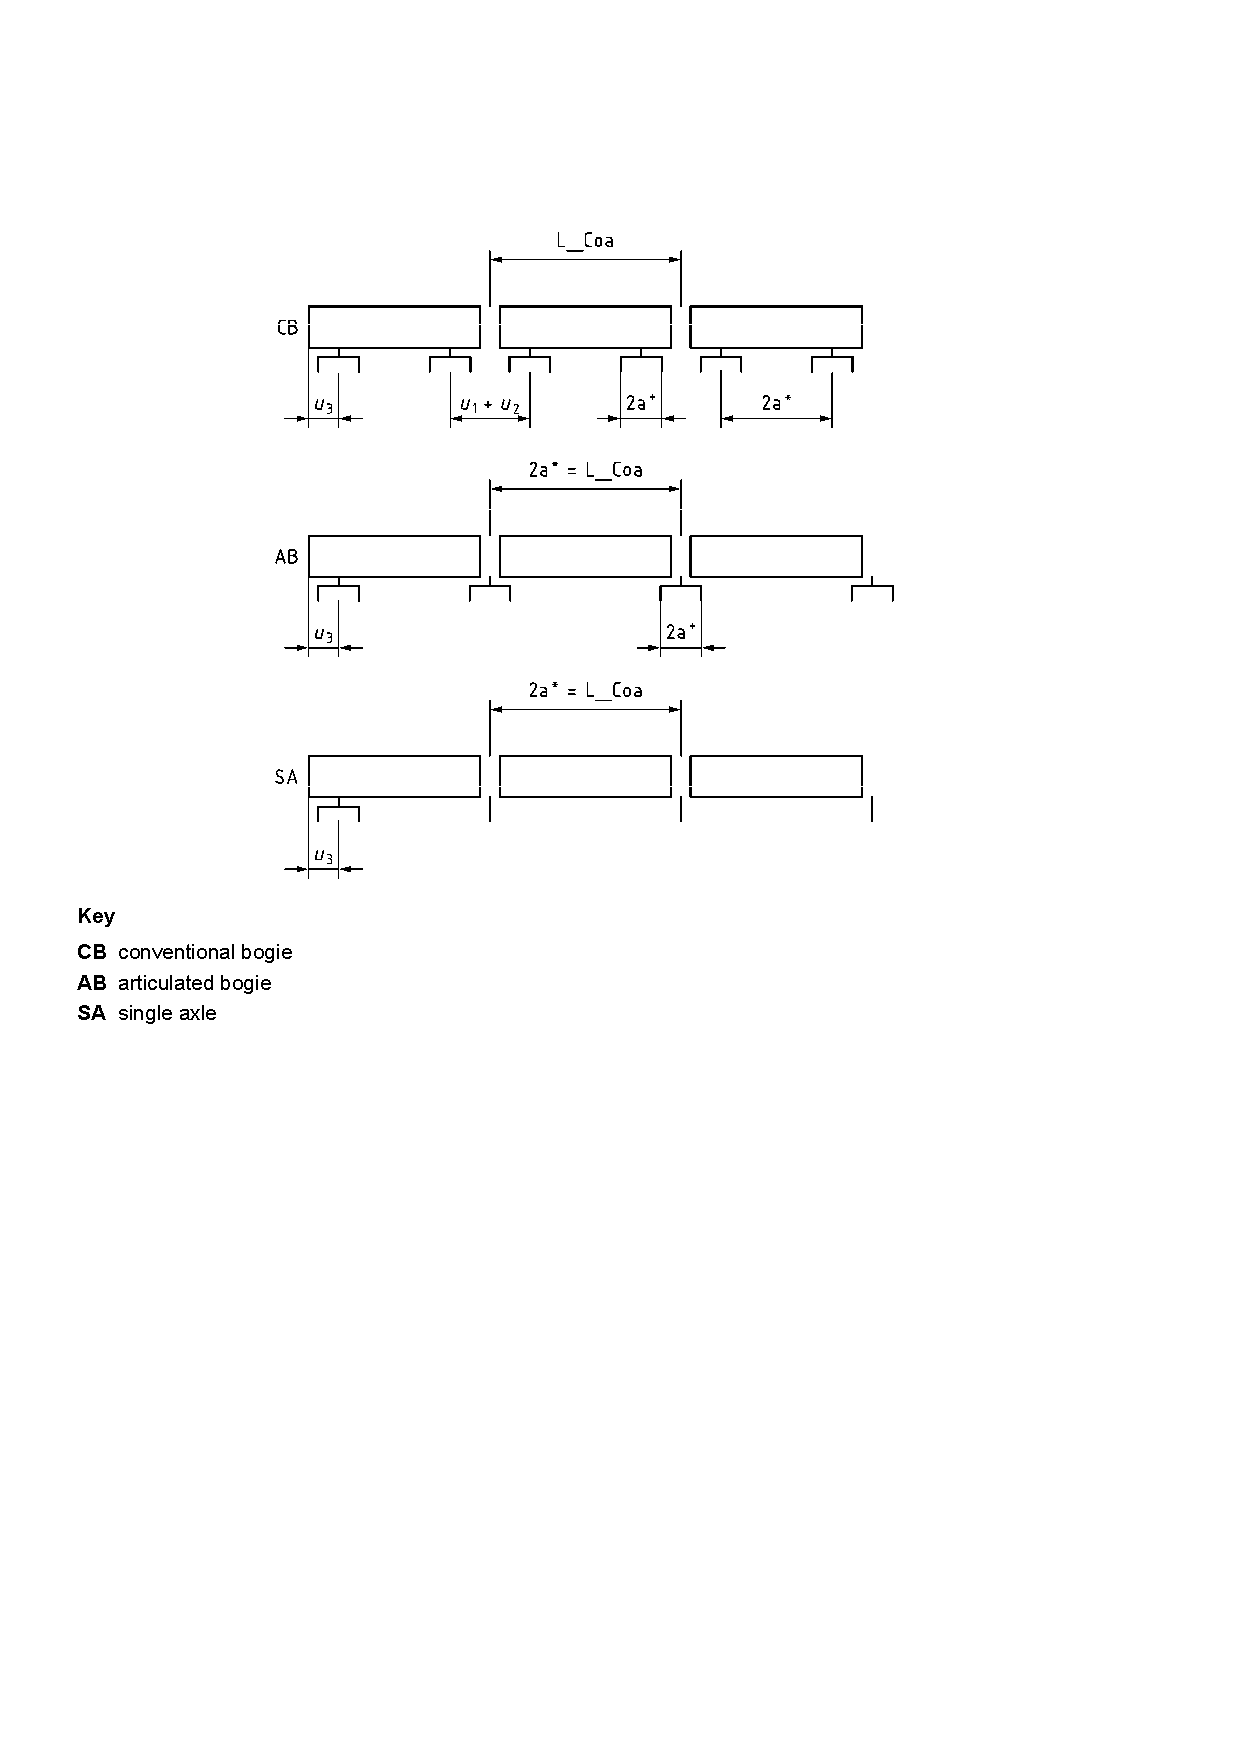
\includegraphics[width=0.8\textwidth]{trainparameters.pdf}
\caption{Train parameters related to MU-Groups. Extracted from \cite[Annex C]{EC15528}}
\label{fig:trainparameters}
\end{figure}

\begin{table}[h]
    \centering
    \begin{tabular}{c|c|c}
    \hline
    Name & Parameter & Unit \\
    $2a^*$ & Bogie spacing between pivot centres within a vehicle & m \\
    $2a^+$ & Axle spacing in bogie & m \\
    $u1+u2$ & Bogie spacing between pivot centres of adjacent vehicles & m \\
    $u3$ & Overhang of end coaches & m \\
    L\_Coa & Coach length & m \\
    No\_Coa & Number of coaches within an unit & - \\
    No\_Units & Number of units within a train & - \\
    \hline
    \end{tabular}
    \caption{Explanation of train parameters. Extracted from \cite[Annex C]{EC15528}}
    \label{tab:explanationtrainparameters}
\end{table}

\subsection{Train parameters of MU-Class CB\_1}

\begin{table}[h]
    \centering
    \begin{tabular}{c|c}
    \hline
    max No\_Units & 2 \\
    max No\_Coa & 8 \\
    L\_Coa & $23.8m \leq L\_Coa \leq 25.3m $ \\
    $2a^*$ & $16.8m \leq 2a^* \leq 18.0m $ \\
    $2a^+$ & $2m \leq 2a^+ \leq 3m $ \\
    $(u1+u2)$ & $7.0m \leq (u1+u2) \leq 7.6m $ \\
    $u3$ & $4m \leq u3 \leq 6m $ \\
    \hline
    \end{tabular}
    \caption{Train parameters for conformity with MU-Class CB\_1}
    \label{tab:CB1}
\end{table}

\subsection{Train parameters of MU-Class CB\_2}

\begin{table}[h]
    \centering
    \begin{tabular}{c|c}
    \hline
    max No\_Units & 2 \\
    max No\_Coa & 7 \\
    L\_Coa & $ 25.3 m \leq L\_Coa \leq 27.5 m $ \\
    $2a^*$ & $ 18.0 m \leq 2a^* \leq 19.5 m $ \\
    $2a^+$ & $ 2 m \leq 2a^+ \leq 3m $ \\
    $(u1+u2)$ & $7.2m \leq (u1+u2) \leq 8.0 m $ \\
    $u3$ & $4m \leq u3 \leq 6m $ \\
    \hline
    \end{tabular}
    \caption{Train parameters for conformity with MU-Class CB\_2}
    \label{tab:CB2}
\end{table}


\subsection{Train parameters of MU-Class AB\_1}

\begin{table}[h]
    \centering
    \begin{tabular}{c|c}
    \hline
    max No\_Units & 4 \\
    max No\_Coa & 5 \\
    $2a^*$ & $ 14.9 m \leq 2a^* \leq 16.0 m $ \\
    $2a^+$ & $ 2 m \leq 2a^+ \leq 3m $ \\
    $u3$ & $3m \leq u3 \leq 5.5m $ \\
    \hline
    \end{tabular}
    \caption{Train parameters for conformity with MU-Class AB\_1}
    \label{tab:AB1}
\end{table}

\subsection{Train parameters of MU-Class AB\_2}

\begin{table}[h]
    \centering
    \begin{tabular}{c|c}
    \hline
    max No\_Units & 4 \\
    max No\_Coa & 5 \\
    $2a^*$ & $ 18.8 m \leq 2a^* \leq 19.5 m $ \\
    $2a^+$ & $ 2 m \leq 2a^+ \leq 3m $ \\
    $u3$ & $3m \leq u3 \leq 5.5m $ \\
    \hline
    \end{tabular}
    \caption{Train parameters for conformity with MU-Class AB\_2}
    \label{tab:AB2}
\end{table}

\subsection{Train parameters of MU-Class AB\_3}

\begin{table}[h]
    \centering
    \begin{tabular}{c|c}
    \hline
    max No\_Units & 2 \\
    max No\_Coa & 11 \\
    $2a^*$ & $ 17.0 m \leq 2a^* \leq 17.5 m $ \\
    $2a^+$ & $ 2 m \leq 2a^+ \leq 3m $ \\
    $u3$ & $4.5m \leq u3 \leq 5.7m $ \\
    \hline
    \end{tabular}
    \caption{Train parameters for conformity with MU-Class AB\_3}
    \label{tab:AB3}
\end{table}

\subsection{Train parameters of MU-Class AB\_4}

\begin{table}[h]
    \centering
    \begin{tabular}{c|c}
    \hline
    max No\_Units & 2 \\
    max No\_Coa & 10 \\
    $2a^*$ & $ 18.7 m \leq 2a^* \leq 19.2 m $ \\
    $2a^+$ & $ 2 m \leq 2a^+ \leq 3m $ \\
    $u3$ & $4.3m \leq u3 \leq 5.3m $ \\
    \hline
    \end{tabular}
    \caption{Train parameters for conformity with MU-Class AB\_4}
    \label{tab:AB4}
\end{table}

\subsection{Train parameters of MU-Class SA\_1}

\begin{table}[h]
    \centering
    \begin{tabular}{c|c}
    \hline
    max No\_Units & 3 \\
    max No\_Coa & 10 \\
    $2a^*$ & $ 9.2 m \leq 2a^* \leq 9.8 m $ \\
    $u3$ & $4.25m \leq u3 \leq 6.25m $ \\
    \hline
    \end{tabular}
    \caption{Train parameters for conformity with MU-Class SA\_1}
    \label{tab:SA1}
\end{table}

\subsection{Train parameters of MU-Class SA\_2}

\begin{table}[h]
    \centering
    \begin{tabular}{c|c}
    \hline
    max No\_Units & 2 \\
    max No\_Coa & 14 \\
    $2a^*$ & $ 12.8 m \leq 2a^* \leq 13.5 m $ \\
    $u3$ & $4.25m \leq u3 \leq 6.25m $ \\
    \hline
    \end{tabular}
    \caption{Train parameters for conformity with MU-Class SA\_1}
    \label{tab:SA1}
\end{table}

\end{appendices}